\chapter{Nuclear Physics}
\section{Rutherford Scattering Experiment}
Nucleus is discovered by Ratherford using alpha particles. Scattering experiment in which they placed a sample of alpha emitting substance behind a lead screen with a small hole in it. So that a narrow beam of alpha particle was produced. This beam was directed at a thin gold foil. A zin sulfide screen, which gives off a visible flash of light when srruck by a alpha particle was set on the side of the foil with microscope to see the flashes. It was expected that alpha particle would go right through the foil with hardly any deflection. But it was found was that although most of the alpha particle indeed were not deviated by much, a few were scattered through very large angles. Rutherford explained the result as an atom as being composed of a tiny nucleus in which its positive charge and all its mass are concentrated with the electrons some distance away with an atom being largely empty space it is easy to see why most alpha particle go right through a thin foil. How ever when an alpha particle heppens to come near a nucleus . The intence electric field there scatteres it through a large angle. The atomic electrons, being so light do not appreciably affect the alpha particles.\\
	\begin{figure}[H]
		\centering
		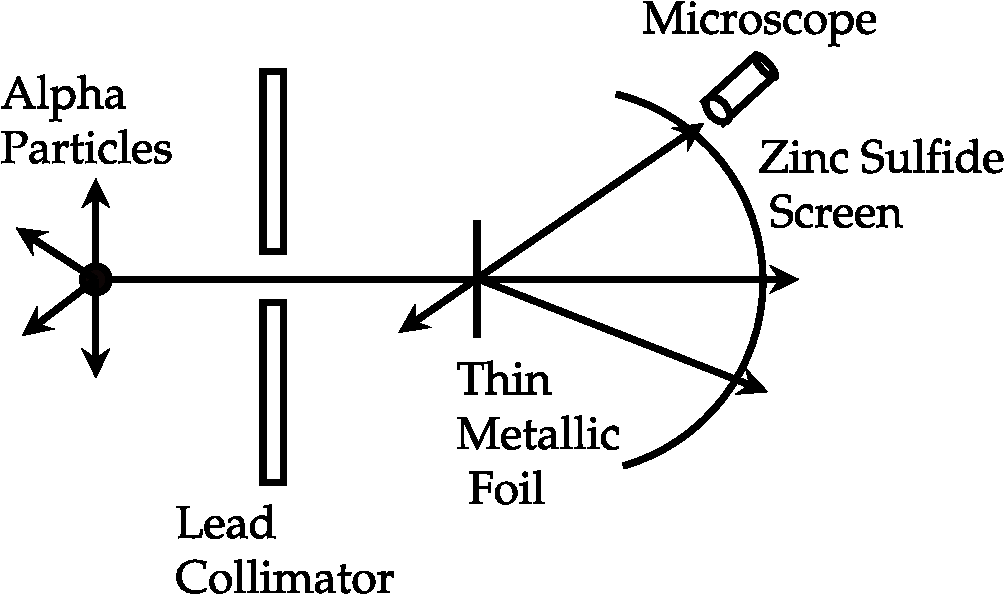
\includegraphics[height=4cm,width=7cm]{58.1-crop}
		\caption{}
		\label{}
	\end{figure}
\subsection{Scattering Formula}
\begin{align*}
N(\theta)&=\frac{N_l nt z^2 e^4}{(8\pi\varepsilon_0)^2r^2(KE)^2\sin^4(\frac{\theta}{2})}\\
N(\theta)&=\text{No of alpha particle per unit area that reach the screen at a scattering angle of $\theta$}\\
N_l&=\text{Total no of alpha particle that reach the screen}\\
n&=\text{No of atoms per unit volume in the foil}\\
z&=\text{Atomic numner of the foil atoms}\\
r&=\text{Distance of the screen from the foil}\\
KE&=\text{Kinetic energy of the alpha particles}\\
t&=\text{Foil thickness}
\end{align*}
\subsection{Nuclear Diamensions}
Rutherford assumed that the size of the target nucleus is small compared with the minimum distance $R$ to which incident alpha particle approch the nucleus before being deflected away. At the instant of closest approch (R), the initial $kE$ of the particle is entirely converted to electric potential energy. So that instant\\
\begin{align*}
KE_{initial}=PE=\frac{1}{4\pi\varepsilon_0}\frac{2ze^2}{R}\\
\text{Charge of alpha particle}&=2e\\
\text{Charge of nucleus}=ze
\end{align*}
\begin{center}
	\framebox{
		\parbox[t][1cm]{3cm}{
			
			\addvspace{-.3cm} \centering
			
			\begin{align*}
			R=\frac{2ze^2}{4\pi\varepsilon_0KE_{Initial}}
			\end{align*}} }
\end{center}
\begin{exercise}
	 Find the distance of closest approch when an alpha particle of $KE7.7 MeV$Scattered by a gold foil.
\end{exercise}
\begin{answer}
\begin{align*}
R&=\frac{2ze^2}{4\pi\varepsilon_0KE_{Initial}}\\
z(gold)&=79\\
R&=\frac{2\times79\times(16\times10^{-19})^2\times9\times10^9}{7.7\times10^6\times1.6\times10^{-19}}\\
R&=3\times10^{-14}m
\end{align*}
Radius of the gold nucleus is therefore lessthan $3\times10^{-14}$	
\end{answer}
\section{Nuclear Compositions}
\begin{enumerate}
\item  \textbf{Nucleons}\\All nucleus are composed of two type of particles positively charged protons and neutral neutrons jointly called as nucleons.
\item \textbf{ Atomic Number (Z)}\\
 Atomic number of an element is the no of protons in each of its atomic nuclei, which is same as the no of electrons in a neutral atom of the element.
 \item \textbf{ Mass Number (A)}\\
 Mass number of the nuclide. Total nubber of nuleons in the nucleus $A=Z+N$ $N$ is the number of neutrons in the atomic nuclens.
 \item \textbf{ Symbol of Nucleus}\\
 $^A_ZX$
 where X=chemical symbol of the element.\\
 Z=atomic number.\\
 A=mass number
 \begin{itemize}
 	\item Even-even nuclei=even proton number(Z), even neutron number $N$
 \item 	Even-odd nuclei=even protone number (Z), odd neutron number $N$
 \item 	Odd-even nuclei=odd protone number (Z), even neutron number $N$
 \item	Odd-odd nuclei=odd protone number (Z), even neutron number $N$.
 \end{itemize}
\item \textbf{Isotopes}\\
Atomic nuclei of the same element have the same number of the protons (Z) but can have different number of neutrons(N)\\
$^A_ZX$ \quad and \quad $^{A+1}_ZX$\quad  are isotopes\\
\textbf{Examples}\\
\textbf{1}\quad $^{13}_6C$\quad and \quad $^{14}_6 C$\\
\textbf{2)}\quad $^1_1H,\quad^2_1H,\quad^3_1H$\\
 Hydrogen deuterium and titrium are the isotops of Hydrogen\\
\begin{figure}[H]
	\centering
	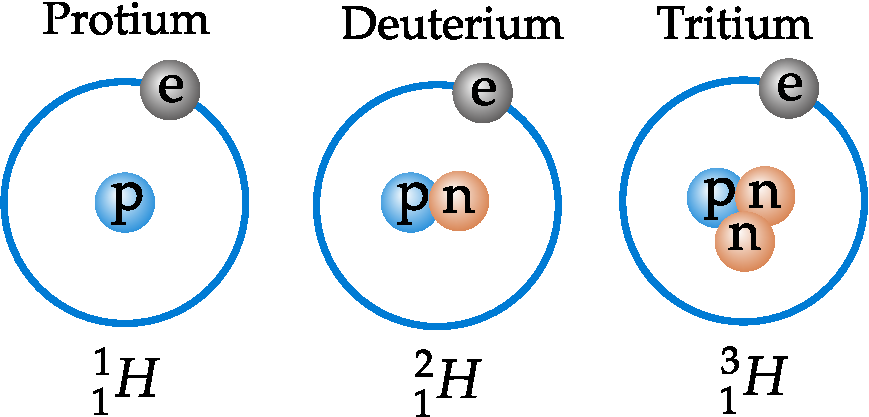
\includegraphics[height=4cm,width=8cm]{20.11-crop}
	\caption{}
	\label{}
\end{figure}
\begin{note}
	\textbf{1)}\quad $^1_2 H$ -\quad deuterium is stable, and is called heavy water\\\\
		\textbf{2)}\quad $^3_1H$-Tritium is radio active, which are found in atmosphere by the nuclear reactions of cosmic rays in the atmosphere.  Only about $2kg$ of tritium is present at any time of earth.
\end{note}
\item  \textbf{Isobars}\\
Atomic nuclei with equal mass number $A$,but different proton number $Z$ .
\begin{itemize}
	\item $^A_Z X$ \  and\ $^A_{Z+1} Y$ are Isobars.
\end{itemize}
\textbf{example}\quad $^{14}C$\  and\  $^{14} N$
\item  \textbf{Isotones}\\
Atomic nuclei with equal neutron numbers but different atomic number $Z$.
\begin{itemize}
	\item $^A_Z X$ \  and\ $^{A+1}_{Z+1} Y$ are Isotons.
\end{itemize}
\item  \textbf{Atomic Masses}\\
Atomic masses refer to the masses of neutral atoms, not of bare nuclei. Thus an atomic mass always include the mass of $Z$ electrons. Atomic mass are expressed in mass units (u). Which is equal to $\frac{1}{12}$ of the mass of neutral atom of \ $^{12}_6 C$\\
$$n=\frac{1}{12} m\left({ }{^{12}_6C}\right)=\frac{1 \mathrm{~g}}{N_{A}}=1.660 \times 10^{-27} \mathrm{~kg} .$$
\begin{center}
	\framebox{
		\parbox[t][0.5cm]{3.5cm}{
			
			\addvspace{-0.5cm} \centering
			
			\begin{align*}
			1 n=1.660 \times 10^{-27} kg
			\end{align*}} }
\end{center}
Where $N_A$ is the avagadro number, equal to $6.023 \times 10^{23}$. Then the mass of $^{12}_6C$ atomic is excatly $12 u$. The energy equalent of mass unit is $931.49 \mathrm{MeV} .$\\\\
\begin{tabular}{c|c|c|c|}
	\hline
	Particle & Mass(Kg) & Mass(u) & Mass($Me V/C^2$)\\
	\hline
	Proton & $1.6726 \times 10^{-27}$ & $1.007276$ & $938 \cdot 28$\\
	\hline
	Neutron & $1.6750 \times10^{-27}$ & $1.008665$ & $939.57 .$\\
	\hline
	Electron & $9.1095 \times 10^{-31}$ & $5.486 \times 10^{-4}$ & $0.511$\\
	\hline
	$^1_1 H$ atom & $1.6736 \times 10^{-27}$ & $1.007825$ & $938.79$\\
	\hline
\end{tabular}\\\\
$\Rightarrow$ \textbf{How to convert mass in $Kg$ in to mass in $u$ and $MeV/C^2$}\\
Take the example as proton with mass $1.6726 \times 10^{-27}$ 
\begin{align*}
\text{Mass in u}&=\frac{1.6726 \times 10^{-27}}{1u}\\
&=\frac{1.6726 \times 10^{-27}}{1.660 \times 10^{-27}}=1.007276u\\
\text{Mass in}\  \frac{\mathrm{MeV}}{C^2} &=1.007276 \times 931.49 \mathrm{MeV}\\
&=938.28 \mathrm{MeV} / \mathrm{c}^{2} 
\end{align*}
\end{enumerate}
\section{Nuclear Properties}
\begin{enumerate}
	\item \textbf{Nuclear charge distribution}\\
 The central nuclear charge density is nearls the same for all nuclei. Nucleons do not seem to congregate near the center of the nucleus. but instead have a fairly constant distribution out to the suriace. Thus the number of nucleons per unit volume is roughly constant:\\
\begin{figure}[H]
	\centering
	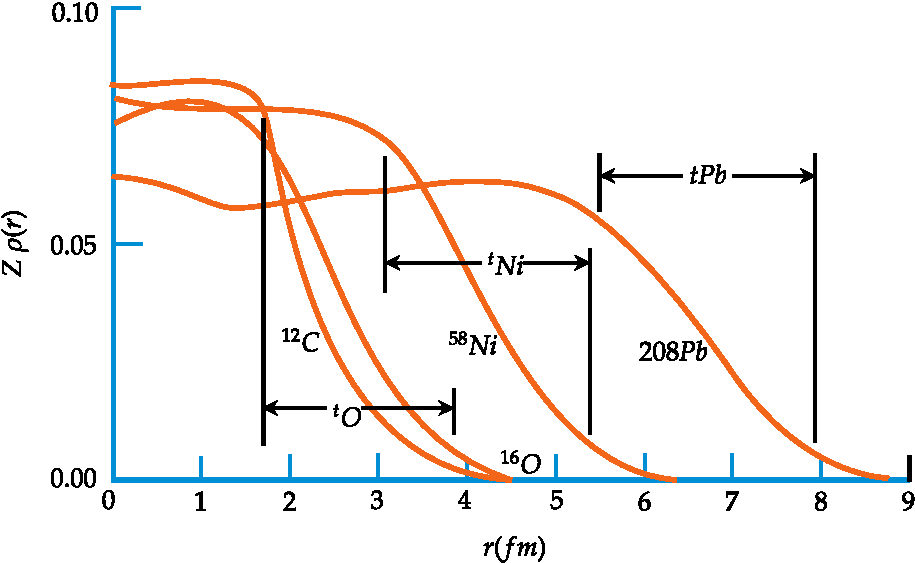
\includegraphics[height=5cm,width=10cm]{diagram-20220307(4)-crop}
	\caption{ The radial charge distribution of several nuciei determined from electron scattering. The skin thickness $t$ is shown for $O, N i$, and $P b$; its value is roughly constant at $2.3 \mathrm{fm}$. The central density changes very littie from the lightest nuclei to the heaviest.}
	\label{ref.nuclear}
\end{figure}
 Figure $\ref{ref.nuclear}$ also shows how diffuse the nuclear surface appears to be. The charge density is roughly constant out to a certain point and then drops relatively slowly to zero. The distance over which this drop occurs is nearly independent of the size of the nucleus, and is usually taken to be constant. We define the skin thickness parameter $t$ as the distance over which the charge density falls from $90 \%$ of its central value to $10 \%$. The value of $t$ is approximately $2.3 \mathrm{fm}$.
	\item \textbf{Size of the Nucleus}\\
It is possible to obtain the size of the nucleus through Ruther ford experiment. We can calculate the size of a nucleus by obtaining the point of closest approach of alpha particle. The size of the nucleus is smaller than $10^{-14}m$. Formula to measure the size of the nucleus can be determined. The volume of the nuclens is proportional to  $A$ \\
\begin{align*}
\frac{4}{3}\pi R^3&\propto A\quad\text{($R$ is the radius) }\\
R&=R_0 A^\frac{1}{3}\\
\text{ Where }R_0&= 1.2\times 10^{-15}m=1.2 fm
\end{align*}
\text{$fm$\ is femtometer (fm)and sometimes called fermi}\\
\textbf{Examples}
\begin{enumerate}
	\item $ \text{Radius of}\ ^{12}_6 C\  \text{nucleus}$
$R\approx(1.2)(12)^\frac{1}{3}fm=2.7fm$
\item $ \text{Radius of }^{107}_{47}Ag$
$R\approx(1.2)(107)^\frac{1}{3}=5.7fm$
 \item $ \text{Radius of }^{238}_{92}u$
$R\approx(1.2)(238)^\frac{1}{3}=7.4fm$
\end{enumerate}
\item \textbf{Density}\\
Density of $^{12}_6C$ nucleus can be find out as
\begin{align*}
\text{Density } \rho &=\frac{mass}{\text { volume. }}\\
\text{Mass of $C$ nuclei is }&=12 u\text{(neglect the masses and binding energies of six electrons)}\\
\rho&=\frac{12\times1.66\times10^{-27}Kg}{\left(\frac{4}{3}\pi \right)\left(2.7\times 10^{-15} m \right)^3  }\\
&=2.4 \times 10^{17} Kg l \mathrm{~m}^{3}
\end{align*}
Which is equalent to 4 billion tones per cubic inch. So it is approximately taken the same for all nuclei.
\begin{center}
	\framebox{
		\parbox[t][0.5cm]{3.5cm}{
			
			\addvspace{-0.5cm} \centering
			
			\begin{align*}
			\text{Density}S=2.4\times10^{17}Kg/m^3
			\end{align*}} }
\end{center}
for all nuclei
\item \textbf{Spin of Nucleus}\\
Proton and neutrons like electrons are fermions with spin quantum number of $S=\frac{1}{2}$
\begin{enumerate}
	\item \textbf{Spin Angular Momenta S(individual)}$\left. \right. $\\
\begin{minipage}{0.45\textwidth}
	\begin{align*}
	S_{p/n}&=\sqrt{S(S+1)}=\sqrt{\frac{1}{2}\left(\frac{1}{2} +1\right) \hbar}\\
	S_{p/n}&=\frac{\sqrt{3}}{2}\hbar\\
	\text{and}\\
	S_z&=m_s\hbar=\pm\frac{1}{2}\hbar
	\end{align*}
\end{minipage}
\begin{minipage}{0.30\textwidth}
	\begin{figure}[H]
		\centering
		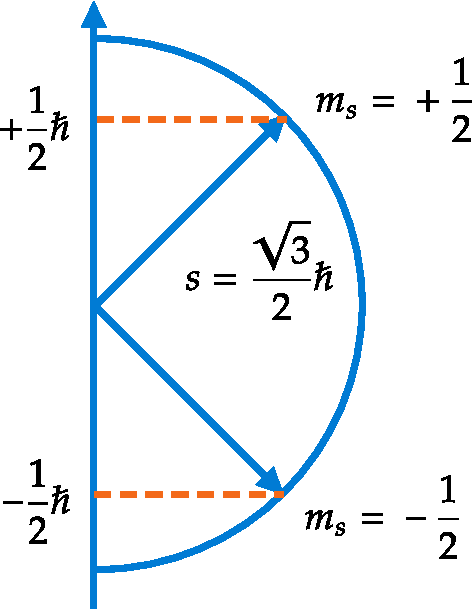
\includegraphics[height=4cm,width=3.5cm]{NC 03-crop}
		\caption{}
		\label{Decreasing Function}
	\end{figure}
\end{minipage}\\
$m_s$ is the spin magnetic quantum number $m_s=\pm\frac{1}{2}$. $S_z$ is $z $ component of spin angular momentum.
 \textbf{Total Spin angular moment of Nucleus}\\
1)\quad Spin of Hydrogen $=\frac{1}{2}$\\\\
2)\quad Nuclei with both $P$and $n$ are even ($A,Z$ even) have total 
Spin $=0$\\
\textbf{Eg:}\quad $^2_2 H,\  ^{12}_6 C,\ ^{16}_8 O$\\\\
3)\quad Nuclei with Both $P$ and $n$\ are odd ($Z$\ odd,\ $A$ even) have 
 integral spin\\
\textbf{Eg:}\quad $^2_1 H,\  ^{14}_7 N,\ ^{10}_5 B$\\\\
4)\quad nuclei With an odd A(mass number) have half integral spin\\
\textbf{Eg:}\quad $^1_1 H,\quad ^{15}_7 N$\ (spin$=\frac{1}{2}$),\quad$^{17}_8 O$(spin$=\frac{5}{2}$)\\\\
Total spin of a nucleus can be represented by letter $I$\\
$\therefore I=\sqrt{I(I+1)}\hbar$\\
$I$ may be zero integral or half integral.\\
 For $I=1$, the possible $I_2$ values are $-1,0,+1$ and can be represented as \\\\
\begin{figure}[H]
	\centering
	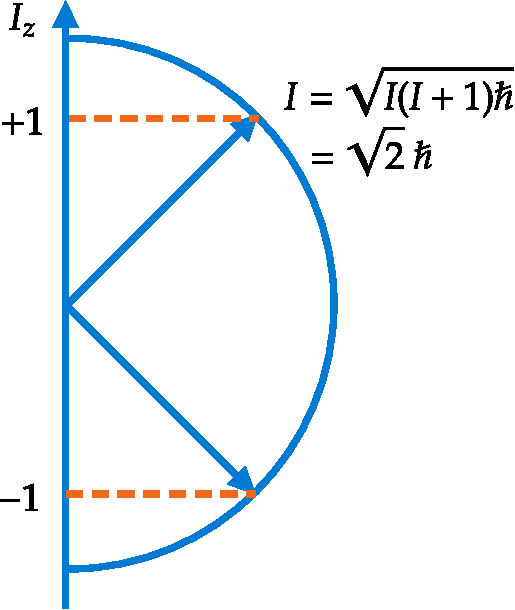
\includegraphics[height=4cm,width=3.5cm]{NC 04-crop}
	\caption{}
	\label{}
\end{figure}
	\item \textbf{Spin Magnetic Momenta(individual)}\\
	 The individual spin magnetic momenta of proton and neutron can be represented as,\\
	\begin{align*}
	\mu_{P_{2}}&=\pm 2.793 \mathrm{N}\\
	\mu_{N_{2}}&=\mp 1..913 \mathrm{N}
	\end{align*}
	The spin magnetic moment $\mu_P$ of the proton is in the same direction as its spin angular momentum. $N$ and in the case of neutron $\mu_{N}$ opposite to $S$.\\\\
	\begin{figure}[H]
		\centering
		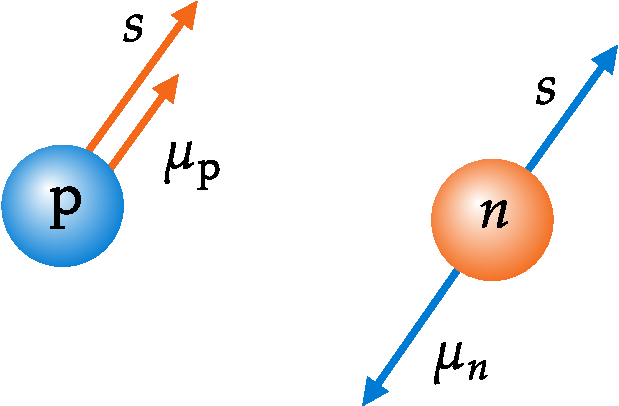
\includegraphics[height=4cm,width=6cm]{CN 05-crop}
		\caption{}
		\label{}
	\end{figure}
\textbf{Total spin magnetic moment of the nucleus}\\
A charged particle spinning about ab axis constitutes a circular electric current which in turn produces a magnetic dipole .In other words the spinning particle behaves as a tiny bar magnet placed along the spin axis.The strength of the magnet for a point charge can be shown to be \\
$$\mu=\frac{q}{2m}I=\frac{q\sqrt{I(I+1)}}{2m}\frac{h}{2\pi}=\frac{qh}{4\pi m}\sqrt{I(I+1)}Am^2$$
We can remove the fiction that nuclei are point charges the above equation become modified by the inclusion of a numerical factor G.\\
$$\mu=\frac{Gqh}{4 \pi m}\sqrt{I(I+1)}JT^{-1}$$
Nuclear G factors cannot be calculated in advance and are obtained only experimentally.\\
Nuclear dipoles are conveniently expressed in terms of nuclear magneton $\beta_N$ which is defined in terms of mass and the charge of the proton.\\
$$\beta_N=\frac{eh}{4m_p \pi}=5.050 \times 10^{-2 7} \mathrm{~J}{T}^{-1}=3.152 \times 10^{-8} \mathrm{eV} T^{-1}$$
Thus for a nucleus of mass M and charge pe(where p is the number of proton)we would write\\
$$\mu=\frac{Gpe}{2M}\sqrt{I(I+1)}\frac{h}{2 \pi}=\frac{Gm_pp}{M}\beta_N\sqrt{I(I+1)}$$
$$=g\beta_N\sqrt{I(I+1)}$$
where we have collected the parameters $\frac{Gm_pp}{M}$ in which $m_p$ is the protonic mass into a factor g which is the characterstics of each nucleus.This factor has value up to about six and is positive for nearlly all known nuclei.\\
The dipole will plainly have components along a reference direction goverened by the $I_z$ values\\
$$\mu_{z}=g\beta_NI_z$$
\end{enumerate}
\begin{note}	
 \textbf{1)}\quad A nucleon in a more complex nucleus may have orbital angular momentum  due to motion inside the nucleus as well as the spin angular momentum. The total angular momenta of such a nucleus is the vector sum of the spin and orbital angular momenta of its nucleus as in the analogous case of the electrons of the atom.\\\\
 	\textbf{2)}\quad \textbf{Larmor Frequency}\\
 	When a nucleus whose magnetic moment has the $Z$ component $\mu_{Z}$ is in a constant magnetic field $B$. The magnetic $PE$ of the nucleus ,\\
 	$$u_{m}=-\mu_{2} B$$
 	Therefore in a magnetic field the angular momentum state of the nucleus is split in to components according to the $m_s$values . Now consider the splitting of angular momenta of the nucleus due to a single proton.\\
 	\begin{figure}[H]
 		\centering
 		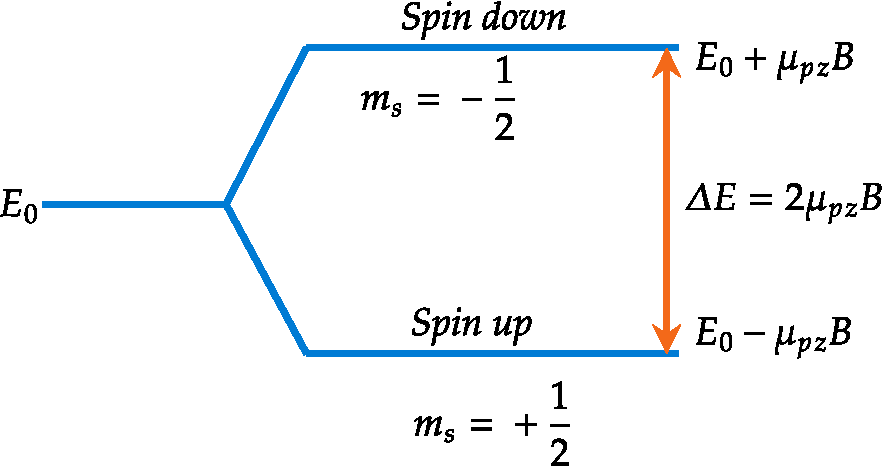
\includegraphics[height=4cm,width=7cm]{CN 06-crop}
 		\caption{}
 		\label{}
 	\end{figure}
 	\begin{align*}
 	B&=0\hspace{2cm} B>0\\
 	\Delta E&=2 \mu_{p_{Z}} B
 	\end{align*}
 	A Proton with this energy will be emitted when a proton in the upper state flips its spin to fall to the lower state. A proton in the lower state can be raised to the upper one by absorbing a photon of the energy. The photon frequency $\nu_L$ that corresponds to $\Delta E$is,\\
 	$$\nu_{L}=\frac{\Delta E}{h}=\frac{2 \mu P_{Z} B}{h}$$
 	This frequency is called Larmor frequency
\end{note}
\begin{exercise}
	 (a)\quad Find the energy difference between the spin up and spin down states of a proton in a magnetic field of $B=1\cdot T$ \\
	(b)\quad What is the Larmor frequency?
\end{exercise}
\begin{answer}
	\begin{align*}
	(a)\quad
	\delta E&=2\mu_{P_{Z}}B=2\times(2.793)\times \left(3.153\times10^-8\frac{eV}{T} \right) \times1T\\
	&=1.761\times10^-7 eV\\
	(b)\quad \nu_{L}&=\frac{\Delta e}{h}=\frac{1.761\times10^{-7}}{4.136\times10^{-15}eV\cdot S}\\
	&=4.258\times10^7Hz=42.58MHz
	\end{align*}
	Which is in the lower end of the microwave part of the spectrum.
\end{answer}
\item \textbf{Electric Moment of Nuclei}
We have seen that the atomic nucleus is a positively charged body of finite dimentions. We know that any distribution of electric charge produce an electric potential $\phi(r,\theta)$at a distance at $r$ in the $Z$ direction. This potential $\phi(r,\theta)$ due to an azimuthally symmetric distribution of electric charges can be expanded in ascending powers of $\frac{1}{r}$
$$\phi(r,\theta)=\frac{1}{r}\sum_{n=o}^{\infty}\frac{a_n}{r^n}P_n(\cos\theta)$$
$P_n$ are the legendre polynomial\\
$I^{st}$ term in the expansion curresponds to potential due to electric monopole. Which is a point charge $+Ze$. The second term corresponds to potential due to electric dipole. But the electric dipole moment of a nucleus is zero for ground state and nondegenerate excited state of the nucleus. Similarly the electric moment of all odd orders (Eg: Octapolemoment)are zeros for the nucleus. The third term in the expansion is called quadrapole moment.
\item \textbf{Electric Quadrapole Moment}\\
Atomic nuclei with spin $=0$ have zero quadrapole moment and sphererical in shape. \\
Atomic nuclei with spin $>1$ have quadrapole moment other than zero. It shows that their form is not strictly spherical. The quadrapole moment has a plus sign if the nucleus is  extended along  the spin axis (a spindle shape body) and minus sign if the nucleus is extented in a plane $\perp$ to the spin axis (a lenticular body). A nucleus posessing a quadrapole moment produces nonspherically symmetrical field. Let $\theta_0$ be the intricsic quadrapole moment of a nucleus. Then 
$$Q_0=\frac{1}{e}\int(3{Z^\prime}^2-{r^\prime}^2)\rho(r^\prime)d\tau^\prime$$
Where integration is carried out over the entire volume of the nucleus. $r^\prime(x^\prime,y^\prime,z^\prime
)$ is the distance measured from the center of mass of the nucleus.\\
For a spherically symmetric charge distribution.
$$\rho(r^\prime){x^\prime}^2d\tau^\prime=\int \rho(r^\prime){y^\prime}^2d\tau^\prime=\int \rho(r^\prime){z^\prime}^2d\tau^\prime=\frac{1}{3}\int \rho(r^\prime){r^\prime}^2d\tau^\prime$$
Therefore $\theta_0=0$for spherical nucleus.\\
For a nonsperical nucleus $\theta$ and $\theta_0$ is related as,
$$Q=Q_0\left( \frac{I(2I-1)}{(I+1)(2I+3)}\right) $$
Where $I$ is the total angular momentum (spin)
$$\text{If}\quad Q_0>0, \int \rho(r^\prime){z^\prime}^2d\tau^\prime>\frac{1}{3}\int \rho(r^\prime){r^\prime}^2d\tau^\prime$$
Such nucleus is eleongated along the $z^\prime$ axis (cigar shaped) is called prolate spheroid.
$$\text{If}\quad Q_0<0, \int \rho(r^\prime){z^\prime}^2d\tau^\prime<\frac{1}{3}\int \rho(r^\prime){r^\prime}^2d\tau^\prime$$
Such nucleus is called oblate spheroid (pancake shape)
\begin{figure}[H]
	\centering
	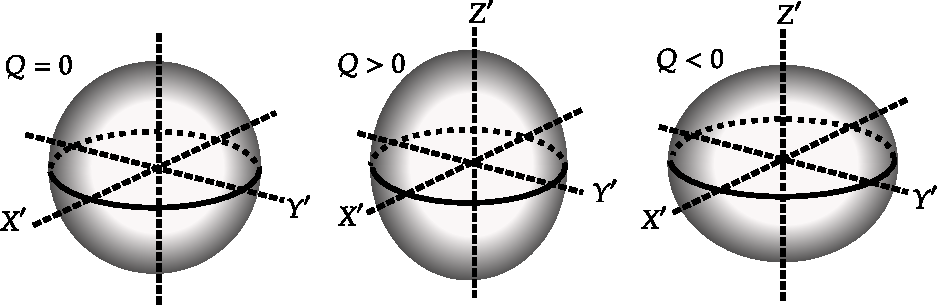
\includegraphics[height=4cm,width=10cm]{diagram-20220307(5)-crop}
	\caption{}
	\label{}
\end{figure}
\end{enumerate}
\section{Binding Energy}
Binding energy $BE$, the energy released when free nucleons are bound together to form a nucleus. SI unit is the Joule(J). Usually the binding energy is given in MeV. The mass of a stable atomic nucleus is smaller than the sum of the masses of the constituent nucleons. The missing mass is converted in to its energy equivalent called binding energy. The greater its $BE$ the more the energy that must be supplied to breake up the nucleus. The binding energy $E_b$in MeV  of the nucleus $^A_ZX$ is given by.
\begin{align*}
E_b&=\left[ zm(^1_1H)+NM(n)-m(^A_ZX)\right]\left(931.49\  MeV/u \right)  \\
\text{Where}\\
m(^1_1H)&=\text{Is the atomic mass of }^1_1H\\
&=1.007825 u\\
Z&= \text{ Atomic number}\\
N&= \text{No of neutrons}\\
M(n)&=\text{Mass of neutron}\\
&=1.008665 u\\
^A_ZX&= \text{Atomic mass of element }X
\end{align*}
\section{Binding Energy Per Nucleon}
The binding energy per nucleon for a given nucleus is an average found by dividing its total binding energy by the no of nucleons it contain. The range for the stable nuclei is from $2.224\ MeV$ for $^2_1H$\ (deuterium)\ to $1640\ MeV$ for $^{209}_{83}B_1$. The binding energy per nucleon for $^2_1H$\ is $\frac{2.2}{2}=1.1MeV/\text{nucleon}$ and for $^{209}_{83}B_1$\ is $\frac{1640}{209}=7.8 MeV/\text{nucleon}$.\\
The graph binding energy per nucleon against number of nucleons (A) is called binding energy curve.
\begin{exercise}
	The binding energy of neon isotope $^2_{10}Ne$\ is $160.647\ MeV$. Find its atomic mass.
\end{exercise}
\begin{answer}
	\begin{align*}
	\text{Here}\quad Z=10\quad N&=10,E_b=160.647 \ MeV\\
	\left[ Zm(^1_1H)+Nm(n)\right] &-\frac{E_b}{931.49}\\
	=19.992 \ u
	\end{align*}
\end{answer}
\subsection{Binding Energy Curve}
\subsubsection{Conclusions Drawn From the Curve}
\begin{figure}[H]
	\centering
	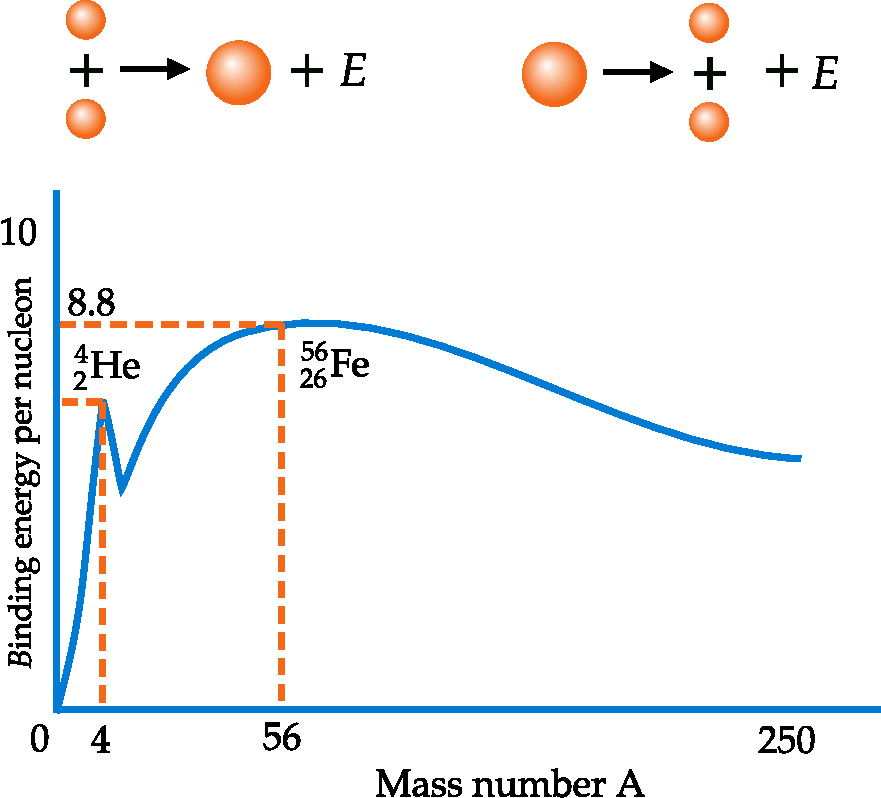
\includegraphics[height=7cm,width=7.5cm]{NC 07-crop}
	\caption{}
	\label{}
\end{figure}
\textbf{1)} \quad Binding energy per nucleons is almost constant except for very small $A$\\
The peak at $A=4$ corresponds to the exceptionally stable $^4_2He$ nucleus. Which is the alpha particle \\\\
\textbf{2)}\quad The graph has its maximum of $8.8\ MeV/\text{nucleon}$. When the total number of neucleon is $56$. That is $^{56}_{26}Fe$\ is $160.647\ MeV$ an iron isotope.\\\\
\textbf{3)}Suppose if we split a heavy nucleus (At the last part of the graph) in to two medium sized ones, each of the nuclei will have more binding energy per nucleon than the original nucleus have. A lot extra energy will be given off.\\\\
\textbf{Eg:}\quad If uranium nucleus $^{235}_{92}U$\ is broken into smaller nuclei. The binding energy difference per nucleon is $0.8\ MeV$\\
Then total energy given off $=0.8\times235=188\ MeV$. A single nucleus can given this much of energy. Which is very large.\\
Such splitting of heavy nucleus in to smaller one with large amount of energy is called nuclear fission.\\\\
\textbf{4)}\quad Suppose that we are joining two light nuclei together to give a single nucleus of medium sized one will also given off large amount of energy.\\\\
\textbf{Eg:} \quad If two $^2_1H$( deuterium )nuclei combine to form a  $^4_2He$\ Helium nucleus about $23MeV$\ energy is released. Such process is called Nuclear Fission. Is the main energy source of the sun and other stars.
\section{Nuclear Models}
We know much about the arrangement of the orbital electron in an atom. This is large because of the force between the electron and the nucleus as well as between electron themselves is electrical in nature and mathematical treatment of such forces is well established. Unfortunately there is no satisfactory explanation for treating the strong nuclear interaction based on the concept of pion transfer. Consequently there is no simple theory of the detailed structure of the nucleus.\\
What physicist have done so for is to propose models which can be used to interpret certain aspects of the behaviour of nuclei. Few of them are\\
(a)\quad Why do nucleus emit $\alpha$ and $\beta$ particles. When there are known to contain only protons and neutrons. \\
(b)\quad Why is binding energy per nucleon almost constant? \\
(c)\quad Why are $4u$ nuclei particularly stable?\\
(d)\quad How one can explain the excited state of nuclei\\
(e)\quad How one can interpret the special properties of nucleus 
Eg:\quad spin, stability magnetic moment etc.\\\\
Various models which have been preposed for the nucleus are the different collective models(of which the liquid drop model is the one), fermi gas model and the shell model with different types of coupling. One can see that the resemblence to a drop of liquid setves us basis for the liquid drop model and collective model and resemblence to a weakly interacting gas serves as the basis for the fermi gas model and the shell model. Liquid drop model and shell model are briefly reviewed in this discussion.  \\
\subsection{Liquid Drop Model}
The binding energies and the volume of the nuclei are proportional to the number of nucleons present in nuclei. The proportionality however indicates the short range and saturation characters of the nuclear force. This follows that there is strong interactions amongst all the neighbouring nucleons inside the nucleus. This properties of a nucleus are analogous to the properties of the force which hold a liquid drop together. This analogy led to prepose the liquid drop model of the nucleus. This model is not considered about the individual characteristics of the nucleons and hence this is a statistical model. According to this model nucleus is regarded as an incompressible and uniformly charged liquid drop.\\
\textbf{(a)\quad similarities Between a Nucleus and Liquid 
Drop}\\
\textbf{(i)}\quad There are large number of particle in a nucleus as in a drop of liquid, protons and neutrons in the former and molecule or atoms in the latter. \\
\textbf{(ii)}\quad Both of the liquid drop and nucleus exhibits homogeneity and incompressibility, for Eg: charge density is almost constant through out the drop and the nucleus. In both cases density is independent of diamensions \\
\textbf{(iii)}\quad Each nucleus in a nuclens interacts strongly with a small number of adjacent nucleons just as do the molecule in a liquid drop. This follows that the nucleon forces are of short range and of saturation character.\\
\textbf{(iv)}\quad Both liquid drop and nucleus show surface tension effect ie the surface energy of the nucleus is analogous to the surface tension of liquids \\
\textbf{(v)}\quad A part  from the coloumb repulsion the forces between the \ $n-n,\ n-p$\ and \ $p-p$\ are the same in the nucleus just as the intermolecular forces in an ideal solution
\textbf{(vi)}\quad Evaporation from a liquid is analogous to the loss of nucleus from a nucleus in the nuclear reaction.\\
\textbf{(vii)}\quad The fusion of small drops in to a bigger one, and the breaking up of large drop into small droplets are quite analogous to the fusion of light nuclei in to a heavy nucleus and the fusion of a heavy nucleus in to a light nuclei respectively. The fusion and fission in both cases are exoergic.\\
\textbf{(viii)}\quad The thermal agitation of the molecules in a drop is quite analogous to the kinetic energy of the nucleons in a nucleus.\\
\textbf{(b)\quad Bethe-Weizsacker Semi-Emperical Mass Formula}\\
On the basis of the liquid drop model, Weiszacker and several others have attempted to express the mass of the nuclei in terms of nuclear characteristics in connection with their binding energy and stability. This formula is known as semi-emperical mass formula. Let \ $m(A,Z)$\ mass of the isotope of an element $X$ of atomic number $Z$ and mass number $A$.Then,
\begin{align*}
m(A,Z)&=ZM_H+NM_n-E_b\\
\text{Where}\\
M_H&=\text{Mass of Hydrogen}\\
M_n&=\text{Mass of Neutron}\\
N=A-Z&=\text{ Number of Neutrons}\\
E_b&=\text{Binding energy}
\end{align*}
\text{One can express the binding energy $E_b$ as the sum of no of terms as bellow.}\\
\textbf{(I)\quad Volume Energy}\\
We start by assuming that the energy associated with each nucleon-nucleon bond has some value $u$. Because each bond energy $u$ is shared by two nucleons. Each has a binding energy of $\frac{1}{2}u$. When an assembly of shares of same size is packet together in to a smallest volume, as we suppose is the case of nucleons with in a nucleus, each interior sphere $12$ other spheres in contact with it. Hence each interior nucleon in a nucleus has a binding  energy of $12(\frac{1}{2}u)=6u$. If all $A$ nucleons in a nucleus were in its interior. The total binding energy of the nucleus would be,
\begin{align*}
E_v&=6Au\\
\text{Volume energy} E_v&=a_1 A\\
E_v&\propto A
\end{align*}
\textbf{(II)\quad Surface Energy}\\
Nucleons on the surface will have less than $12$ neighbours in contacts. since we have included all nucleons (A) in volume energy we have to minus the energy of peripheral nucleons which is called surface energy. A nucleus with radius $R$ has surfice are $4\pi R^2(4\pi R^2_0A^\frac{2}{3})$. So surface energy is preportional to $(4\pi R^2_0A^\frac{2}{3}) $\\
\begin{align*}
E_s\alpha-\frac{4}{3}\pi R^2_0A^\frac{2}{3}\\
E_s=-a_2 A^\frac{2}{3}
\end{align*}
For a nucleus to be stable binding energy should be maximum. So the surface energy term would be a small quantity. For a given volume sphere has the least surface area. So the nucleus size will be spherical and should exhibit the same surface tension effect as a liquid drop.\\
\textbf{(III)\quad Coloumb Energy}\\
Electric repulsion between each pair of proton in a nucleus also contributes towards decreasing its binding energy. The columb energy $Ec$ of a nucleus is the work that must be done to bring $Z$ protons from infinity in to a spherical aggregate the size of the nucleus.
\begin{align*}
\intertext{The potential energy of a pair of protons $r$ a part,}
V&=\frac{-e^2}{4\pi\varepsilon_0 r}
\intertext{Since there are  $\frac{Z(Z-1)}{2}$ pairs of protons}
E_c=\frac{Z(Z-1)}{2}V&=\frac{-Z(Z-1)e^2}{4\pi\varepsilon_0}\left( \frac{1}{r}\right)_{av}
\intertext{If the protons are uniformly distributed through out a nucleus of radius $R$}
\intertext{$\left( \frac{1}{r}\right)_{av}$ is proportional to $\left( \frac{1}{R}\right)$and hence $\frac{1}{A^\frac{1}{3}}$}
\text{Coloumb energy}E_c&=-a_3\frac{Z(Z-1)}{A^\frac{1}{3}}
\intertext{The coloumb energy is negative because it arises from the effect that opposes nuclear stability.}
\intertext{The total binding energy $E_b$ of the nucleus is the sum of $E_v,\ E_s,\ $and $\ E_c$ }
E_b&=E_v+E_s+E_c\\
&=a_1A-a_zA^\frac{2}{3}-a_3\frac{Z(Z-1)}{A^\frac{1}{3}}
\intertext{Binding energy nucleon}
\frac{E_b}{A}&=a_1-\frac{a_2}{A^\frac{1}{3}-a_3\frac{z(z-1)}{A^\frac{4}{3}}}
\intertext{When we plot,}
\end{align*}
\begin{figure}[H]
	\centering
	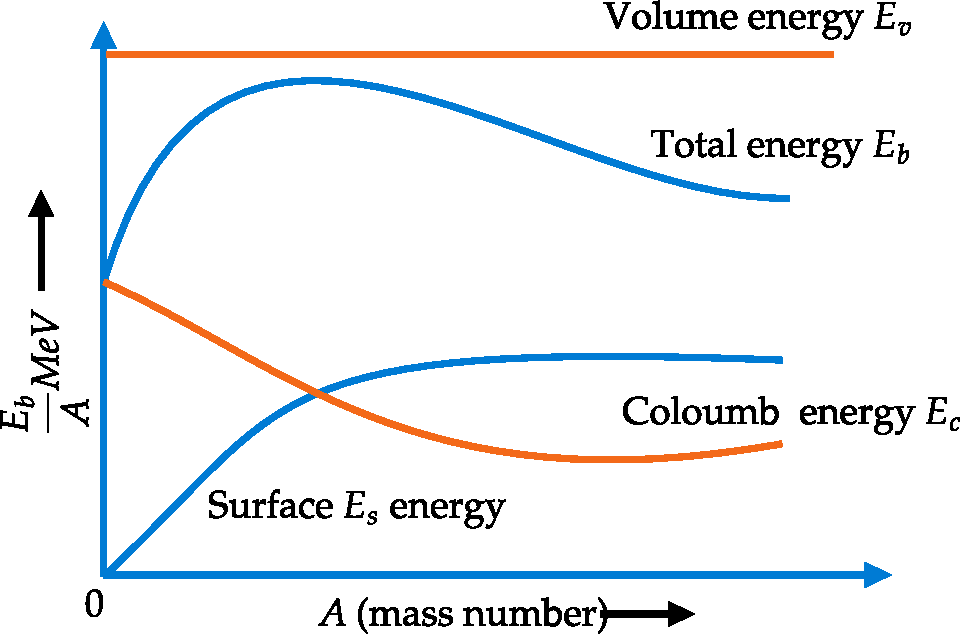
\includegraphics[height=5cm,width=7cm]{NC 08-crop}
\end{figure}
\subsection{Shell model}
\subsubsection{Evidence of shell structure}
\begin{enumerate}
	\item Just as intert gases, with $Z=2,10,18,36,54, \ldots$ electrons having closed shells show high chemical stability, nuclei with $Z=2,8,20,28,50,82$, and 126 nucleons - the so-called magic numbers of the same kind (either proton or neutron) are particularly stable. (Nuclei with $Z=N$, a magic number are said to be doubly magic and show exceptionally high stability).
	\item The number of stable isotopes $(Z=$ const. $)$ and isotones $(N=$ const. $)$ is larger with respective number of protons and neutrons and equal to either of magic numbers, e.g. $S_{n}(Z=50)$ has 10 stable isotopes, $\mathrm{Ca}(Z=20)$ has 6 ; the biggest group of isotone is at $N=82$, then at $N=50$ and $N=20$. The relative abundances of naturally occurring isotopes whose nuclei contain magic numbers of protons or neutrons, have greater relative abundances, e.g. the isotopes ${ }^{88} \mathrm{Sr}(N=50),{ }^{138} \mathrm{Ba}(N=$ $82)$ and ${ }^{140} \mathrm{Ce}(N=82)$ have relative abundances of $82.56 \%, 71.66 \%$ and $88.48$ \% respectively.
	\item The three naturally occurring radioactive series decay to the stable end product the three isotopes of $\mathrm{Pb} ;{ }_{82}^{206} \mathrm{~Pb}(Z=82, N=124)$, ${ }_{8}^{207} \mathrm{~Pb}(Z=82, N=125)$ and ${ }_{82}^{208} \mathrm{~Pb}$ (with $Z=$ 82 and $N=126$ ) indicating extra stable configuration of magic nuclei.
	\item The neutron absorption cross-section is low for nuclei with $N=$ magic numbers, e.g. 50 , 82 and 126 , indicating reluctance of magic nuclei to accept extra neutrons in their completely filled shells.
	\item Isotopes like ${ }_{8}^{17} \mathrm{O},{ }_{36}^{87} \mathrm{~K}$ and ${ }_{54}^{137} \mathrm{Xe}$ are spontaneous neutron emitters when excited by preceding $\beta$-decay. These isotopes have $N=9,51$ and 83 respectively, i.e., $N(8+1), N(50+1)$ and $N(82+1)$. We can interpret this loosely bound neutron as a valence neutron which the isotopes emit to assume some magic number $N$-value for stability.
	\item Nuclei with magic numbers of neutrons or protons have their first excited states at higher energies than in cases of the neighbouring nuclei.
	\item Electric quadrupole moment $Q$ of magic nuclei is zero indicating spherical symmetry of nucleus for closed shells. When $Z$-value or $N$-value is gradually increases from one magic number to the next, $Q$ increases from zero to a maximum and then decreases to zero at the next magic number.
	\item The energy of $\alpha-$ or $\beta$ - particles emitted by magic radioactive nuclei is larger.
	\item The asymmetry of the fission of the uranium nucleus could involve the sub-structure of nuclei, which is expressed in the existence of the magic numbers.
\end{enumerate}
	\subsubsection{Shell theory}
	The shell model of the nucleus is an attempt to account for the existence of magic numbers and certain other nuclear properties in terms of nucleon behavior in a common force field.\\
	Because the precise form of the potential-energy function for a nucleus is not known, unlike the case of an atom, a suitable function $U(r)$ has to be assumed. A reasonable guess on the basis of the nuclear density curves is a square well with rounded comers. Schrödinger's equation for a particle in a potential well of this kind is then solved, and it is found that stationary states of the system occur that are characterized by quantum numbers $n, l$, and $m_{l}$ whose significance is the same as in the analogous case of stationary states of atomic electrons. Neutrons and protons occupy separate sets of states in a nucleus because the latter interact electrically as well as through the specifically nuclear charge. However, the energy levels that come from such a calculation do not agree with the observed sequence of magic numbers. Using other potential-energy functions, for instance that of the harmonic oscillator, gives no better results. Something essential is missing from the picture.\\
	The problem was finally solved independently by Maria Goeppert-Mayer and J. H. D. Jensen in 1949. They realized that it is necessary to incorporate a spin-orbit interaction whose magnitude is such that the consequent splitting of energy levels into sublevels is many times larger than the analogous splitting of atomic energy levels.\\
	\textbf{Assumptions of shell theory}
	\begin{enumerate}
		\item  $L S$ coupling holds only for the very lightest nuclei, in which the $l$ values are necessarily small in their normal configurations. In this scheme , the intrinsic spin angular momenta $S_{i}$ of the particles concerned (the neutrons form one group and the protons another) are coupled together into a total spin momentum $\mathrm{S}$. The orbital angular momenta $\mathrm{L}_{i}$ are separately coupled together into a total orbital momentum $\mathbf{L}$. Then $S$ and $L$ are coupled to form a total angular momentum $\mathbf{J}$ of magnitude $\sqrt{\mathbf{J}(\mathbf{J}+1)} \hbar$.
		\item After a transition region in which an intermediate coupling scheme holds, the heavier nuclei exhibit $j j$ coupling. In this case the $S_{i}$ and $L_{i}$ of each particle are first coupled to form a $\mathbf{J}_{i}$ for that particle of magnitude $\sqrt{j(j+1)} \hbar$. The various $\mathbf{J}_{i}$ then couple together to form the total angular momentum $\mathrm{J}$. The $\mathrm{jj}$ coupling scheme holds for the great majority of nuclei.
		\item The levels are designated by a prefix equal to the total quantum number $n$, a letter that indicates $l$ for each particle in that level according to the usual pattern $(s, p, d, f, g, . .$ corresponding, respectively, to $l=0,1,2,3,4, \ldots$ ), and a subscript equal to $j$.
		\item The spin-orbit interaction splits each state of given $j$ into $2 j+1$ substates, since there are $2 j+1$ allowed orientations of $J_{i}$.
		\item The number of available nuclear states in each nuclear shell is, in ascending order of energy, $2,6,12,8,22$, 32 , and 44. Hence shells are filled when there are 2, 8, 20, 28, 50, 82, and 126 neutrons or protons in a nucleus.
	\end{enumerate}
When an appropriate strength is assumed for the spin-orbit interaction, the energy levels of either class of nucleon fall into the sequence shown in table.
\begin{table}[H]
	\centering
	\renewcommand*{\arraystretch}{1.2}
	\begin{tabular}{|p{2cm}| p{5cm}|p{2cm}|p{2cm}|p{2.5cm}|}
		\hline	
Shell number&State in a Shell&Number of Particles in a Shell&Total Particles upto the Shell Closure\\
\hline
1&$1 s_{\frac{1}{2}}$&2&2\\
2&$1 p_{\frac{3}{2}}, 1 p_{\frac{1}{2}}$&6&8\\
3&$1 d_{\frac{5}{2}}, 2 s_{\frac{1}{2}}, 1 d_{\frac{3}{2}}$&12&20\\
3a&$1 f_{\frac{7}{2}}$&8&28\\
4&$2 p_{\frac{3}{2}}, 1 f_{\frac{5}{2}}, 2 p_{\frac{1}{2}}, 1 g_{\frac{9}{2}}$&22&50\\
5&$1 g_{\frac{7}{2}}, 2 d_{\frac{5}{2}}, 2 d_{\frac{3}{2}}, 3 s_{\frac{1}{2}}, 1 h_{\frac{11}{2}}$&32&82\\
6&$1 h_{\frac{9}{2}}, 2 f_{\frac{7}{2}}, 2 f_{\frac{5}{2}}, 3 p_{\frac{3}{2}}, 3 p_{\frac{1}{2}}, 1 i_{\frac{13}{2}}$&44&126\\
7&$2 g_{\frac{9}{2}}, 3 d_{\frac{5}{2}}, 1 i_{\frac{11}{2}}, 2 g_{\frac{7}{2}}, 4 s_{\frac{1}{2}}, 3 d_{\frac{3}{2}}, 1 j_{\frac{15}{2}}$&58&184\\
\hline
	\end{tabular}
\end{table}
\subsection{Prediction of the shell model}
The shell model accounts for several nuclear phenomena in addition to magic numbers.The shell model can also predict nuclear angular momenta. In even-even nuclei, all the protons and neutrons should pair off to cancel out one another's spin and orbital angular momenta. Thus even-even nuclei ought to have zero nuclear angular momenta, as observed. In even-odd and odd-even nuclei, the half-integral spin of the single "extra" nucleon should be combined with the integral angular momentum of the rest of the nucleus for a half-integral total angular momentum. Odd-odd nuclei each have an extra neutron and an extra proton whose half-integral spins should yield integral total angular momenta. Both these predictions are experimentally confirmed.
\subsubsection{(i)Spin and parity from shell model}
Nuclear states have an intrinsic spin and a well defined parity, $\eta=\pm 1$, defined by the behaviour of the wavefunction for all the nucleons under reversal of their coordinates with the centre of the nucleus at the origin.
$$
\Psi\left(-\mathbf{r}_{1},-\mathbf{r}_{2} \cdots-\mathbf{r}_{\mathbf{A}}\right)=\eta \Psi\left(\mathbf{r}_{1}, \mathbf{r}_{2} \cdots \mathbf{r}_{\mathbf{A}}\right)
$$
The spin and parity of nuclear ground states can usually be determined from the shell model. Protons and neutrons tend to pair up so that the spin of each pair is zero and each pair has even parity $(\eta=1)$. Thus we have
\begin{itemize}
	\item Even-even nuclides (both $\mathrm{Z}$ and $\mathrm{A}$ even) have zero intrinsic spin and even parity.
	\item Odd A nuclei have one unpaired nucleon. The spin of the nucleus is equal to the $j$ value of that unpaired nucleon and the parity is $(-1)^{l}$, where $l$ is the orbital angular momentum of the unpaired nucleon.\\
	For example ${ }_{22}^{47} \mathrm{Ti}$ (titanium) has an even number of protons and 25 neutrons. 20 of the neutrons fill the shells up to magic number 20 and there are 5 in the $1 f_{\frac{7}{2}}$ state $\left(l=3, j=\frac{7}{2}\right)$ Four of these form pairs and the remaining one leads to a nuclear spin of $\frac{7}{2}$ and parity $(-1)^{3}=-1$.
	\item Odd-odd nuclei. In this case there is an unpaired proton whose total angular momentum is $j_{1}$ and an unpaired neutron whose total angular momentum is $j_{2}$. The total spin of the nucleus is the (vector) sum of these angular momenta and can take values between $\left|j_{1}-j_{2}\right|$ and $\left|j_{1}+j_{2}\right|$ (in unit steps). The parity is given by $(-1)^{\left(l_{1}+l_{2}\right)}$, where $l_{1}$ and $l_{2}$ are the orbital angular momenta of the unpaired proton and neutron respectively.\\
	For example ${ }_{3}^{6} \mathrm{Li}$ (lithium) has 3 neutrons and 3 protons. The first two of each fill the $1 s$ level and the thrid is in the $1 p_{\frac{3}{2}}$ level. The orbital angular mometum of each is $l=1$ so the parity is $(-1) \times(-1)=+1$ (even), but the spin can be anywhere between 0 and $3 .$
\end{itemize}
\textbf{Examples}\\
\begin{enumerate}
	\item The level configurations for the simple odd proton nuclei ${ }_{3}^{7} \mathrm{Li}_{4}$ and ${ }_{7}^{15} \mathrm{~N}_{8}$ in their ground states is as follows:\\
	\begin{align*}
		&{ }_{3}^{7} \mathrm{Li}_{4}:\left({ }^{1 s_{\frac{1}{2}}}\right)^{2},\left(1 p_{\frac{3}{2}}\right)^{1} \\
		&{ }_{7}^{15} \mathrm{~N}_{8}:\left({ }^{1 s_{\frac{1}{2}}}\right)^{2},\left(1 p_{\frac{3}{2}}\right)^{4},\left({ }^{1 p_{\frac{1}{2}}}\right)^{1}
	\end{align*}
	After putting pairs of particles in the earlier shells, one finds that they give rise to spins of lass odd protons as $\frac{3}{2}$ and $\frac{1}{2}$ respectively. One obtains the parities of both states as $(-1)^{l}$ and is odd (-) since $l=1$ for the last odd protons in both the examples. Thus the states can be specified as $I^{\pi}$ equals to $\frac{3^{-}}{2}$ and $\frac{1^{-}}{2}$ respectively.
	\item We now consider another example of odd neutron nuclei, ${ }^{33} \mathrm{~S}_{17}$ and ${ }^{29} \mathrm{Si}_{15}$ having following neutron level configurations:\\
	\begin{align*}
	&{ }_{16}^{33} \mathrm{~S}_{17}:\left({ }^{1 s_{\frac{1}{2}}}\right)^{2}\left|\left(1 p_{\frac{3}{2}}\right)^{4}\left({ }^{1 p_{\frac{1}{2}}}\right)^{2}\right|\left({ }^{1 d_{\frac{5}{2}}}\right)^{6}\left({ }^{2 s_{1}} \frac{1}{2}\right)^{2}\left({ }^{29} d_{\frac{3}{2}}\right)^{1} \\
	&{ }_{14}^{2} \mathrm{Si}_{15}:\left({ }^{1 s_{1}} \frac{1}{2}\right)^{2}\left|\left({ }^{1} p_{\frac{3}{2}}\right)^{4}\left({ }^{1 p_{\frac{1}{2}}}\right)^{2}\right|\left({ }^{1 d_{\frac{5}{2}}^{2}}\right)^{6}\left({ }^{2 s_{1}} \frac{1}{2}\right)^{1}
	\end{align*}
	$\text { and have spins } \frac{3}{2} \text { and } \frac{1}{2} \text { respectively. }$
	\item Let us now take the example of mirror nuclei, ${ }^{13} \mathrm{C}_{7}$ and ${ }^{13} \mathrm{~N}_{6}$. The level configuration for 7 odd protons in ${ }^{13} \mathrm{~N}_{6}$ or 7 odd neutrons in ${ }^{13} \mathrm{C}_{7}$ is the same and is expressed as\\
	$$
	\left({ }^{1 s_{1}}\right)^{2},\left(1 p_{\frac{3}{2}}\right)^{4},\left(1 p_{\frac{1}{2}}\right)^{1}
	$$
	Both have same spin $\frac{1}{2}^{-}$as predicted by the shell model and confirmed experimentally. There is another example of mirror nuclei ${ }_{8}^{17} \mathrm{O}_{9}$ and ${ }_{9}^{17} \mathrm{~F}_{8}$. The configuration for both these for the odd neutron or odd proton as\\
	$$
	\left(\begin{array}{c}
	1 s_{\frac{1}{2}}
	\end{array}\right)^{2}\left|\left(1 p_{\frac{3}{2}}\right)^{4}\left(1 p_{\frac{1}{2}}\right)^{2}\right|\left(1 d_{\frac{5}{2}}\right)^{1}
	$$
	Shell model predicts spin $\frac{5}{2}^{+}$for both these mirror nuclei, which is in accordance with the experiment.\\
\end{enumerate}
\textbf{(ii) Magnetic Dipole Moments}
Since nuclei with an odd number of protons and/or neutrons have intrinsic spin they also in general possess a magnetic dipole moment.

The unit of magnetic dipole moment for a nucleus is the "nuclear magneton" defined as\\
$$\mu_{N}=\frac{e \hbar}{2 m_{p}}$$
which is analogous to the Bohr magneton but with the electron mass replaced by the proton mass. It is defined such that the magnetic moment due to a proton with orbital angular momentum  is $\mu_{N} $.
Experimentally it is found that the magnetic moment of the proton (due to its spin) is
$$
\mu_{p}=2.79 \mu_{N}=5.58 \mu_{N} s, \quad\left(s=\frac{1}{2}\right)
$$
and that of the neutron is
$$
\mu_{n}=-1.91 \mu_{N}=-3.82 \mu_{N} s, \quad\left(s=\frac{1}{2}\right)
$$
If we apply a magnetic field in the $z$-direction to a nucleus then the unpaired proton with orbital angular momentum $\mathbf{l}$, spin $\mathbf{s}$ and total angular momentum $\mathbf{j}$ will give a contribution to the $z-$ component of the magnetic moment
$$
\mu^{z}=\left(5.58 s^{z}+l^{z}\right) \mu_{N} .
$$
As in the case of the Zeeman effect, the vector model may be used to express this as
$$
\mu^{z}=\frac{(5.58<\mathbf{s} \cdot \mathbf{j}>+<\mathbf{l} \cdot \mathbf{j}>)}{<\mathbf{j}^{2}>} j^{z} \mu_{N}
$$
using
$$
\begin{aligned}
<\mathbf{j}^{2}>&=j(j+1) \hbar^{2} \\
<\mathbf{s} \cdot \mathbf{j}>&=\frac{1}{2}\left(<\mathbf{j}^{2}>+<\mathbf{s}^{2}>-<\mathbf{l}^{2}>\right) \\
&=\frac{\hbar^{2}}{2}(j(j+1)+s(s+1)-l(l+1)) \\
<\mathbf{l} \cdot \mathbf{j}>&=\frac{1}{2}\left(<\mathbf{j}^{2}>+<\mathbf{l}^{2}>-<\mathbf{s}^{2}>\right) \\
&=\frac{\hbar^{2}}{2}(j(j+1)+l(l+1)-s(s+1))
\end{aligned}
$$
We end up with expression for the contribution to the magnetic moment
$$
\mu=\frac{5.58(j(j+1)+s(s+1)-l(l+1))+(j(j+1)+l(l+1)-s(s+1))}{2 j(j+1)} j \mu_{N}
$$
and for a neutron with orbital angular momentum $l^{\prime}$ and total angular momentum $j^{\prime}$ we get (not contribution from the orbital angular momentum because the neutron is uncharged)
$$
\mu=-\frac{3.82\left(j^{\prime}\left(j^{\prime}+1\right)+s(s+1)-l^{\prime}\left(l^{\prime}+1\right)\right)}{2 j^{\prime}\left(j^{\prime}+1\right)} j^{\prime} \mu_{N}
$$
Thus, for example if we consider the nuclide ${ }_{3}^{7} \mathrm{Li}$ for which there is an unpaired proton in the $2 p_{\frac{3}{2}}$ state $\left(l=1, j=\frac{3}{2}\right.$ then the estimate of the magnetic moment is
$$
\mu=\frac{5.58\left(\frac{3}{2} \times \frac{5}{2}+\frac{1}{2} \times \frac{3}{2}-1 \times 2\right)+\left(\frac{3}{2} \times \frac{5}{2}+1 \times 2-\frac{1}{2} \times \frac{3}{2}\right)}{2 \times \frac{3}{2} \times \frac{5}{2}} \frac{3}{2}=3.79 \mu_{N}
$$
The measured value is $3.26 \mu_{N}$ so the estimate is not too good. For heavier nuclei the estimate from the shell model gets much worse.\\
The precise origin of the magnetic dipole moment is not understood, but in general they cannot be predicted from the shell model. For example for the nuclide ${ }_{9}^{17} \mathrm{~F}$ (fluorine), the measured value of the magnetic moment is $4.72 \mu_{N}$ whereas the value predicted form the above model is $-0.26 \mu_{N}$. !! There are contributions to the magnetic moments from the nuclear potential that is not well-understood.
\section{Radioactivity}
Many nuclides present in the universe are unstable and spondaneously change in to other nuclides by a process pulled radioactive decay. The phenomina is known as radioactivity and was discovered Antonine Bequerel. Following three aspects of radioactivity are extraordinary from the perspective of classical physics.\\
(i) \quad When a nucleus undergo $\alpha$ or $\beta$ decays its atomic number $Z$ changes and it becomes the nucleus of a different form. Obviously the elements are not immutable. (not transformed to the original one naturally)\\
(ii)\quad The energy liberated during radioactive decay comes from with in the individual nuclei without external excitation.\\
(iii)\quad Radioactive decay is statistical process.
\subsection{Radioactive decay}
There are five different ways in which a radio action nuclide can decay . That are by emitting an alpha ($ ^4_2He$ nuclei), beta(electrons),gamma(high energy photons) particles or by positron emission  and electron capture. In which alpha particle is +vely charged and $P$ particles are -vely charged and the gamma rays are natural. The penitrating power is maximum for  gamma rays. The penitrating power of $\alpha$,$\beta$,$\gamma$, particle can be picturized as\\
\begin{figure}[H]
	\centering
	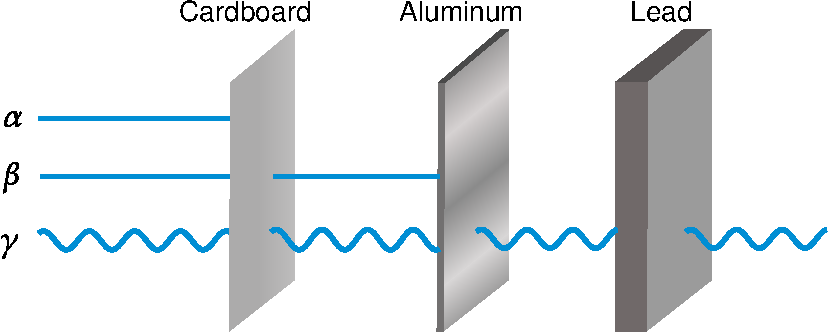
\includegraphics[height=3cm,width=8cm]{diagram-20220307(6)-crop}
	\caption{}
	\label{}
\end{figure}
 Radioactive Decay\\
\begin{tabular}{lll}
	\hline Decay & Transformation & Example \\
	\hline Alpha decay & ${ }_{2}^{A} X \rightarrow{ }_{Z-2}^{A-4} Y+{ }_{2}^{4} \mathrm{He}$ & ${ }_{29}^{238} \mathrm{U} \rightarrow{ }_{90}^{234} \mathrm{Th}+{ }_{2}^{4} \mathrm{He}$ \\
	Beta decay & ${ }_{2}^{A} X \rightarrow{ }_{Z+1}^{A} Y+e^{-}$ & ${ }_{6}^{14} \mathrm{C} \rightarrow{ }_{7}^{14} \mathrm{~N}+e^{-}$ \\
	Positron emission & ${ }_{2}^{A} X \rightarrow{ }_{-1}^{A} Y+e^{+}$ & ${ }_{29}^{64} \mathrm{Cu} \rightarrow{ }_{28}^{64} \mathrm{Ni}+e^{+}$ \\
	Electron capture & ${ }_{Z}^{A} X+e^{-} \rightarrow_{z-1}^{A} Y$ & ${ }_{64}^{A} \mathrm{Cu}+e^{-} \rightarrow{ }_{28}^{64} \mathrm{Ni}$ \\
	Gamma decay & ${ }_{Z}^{A} X^{*} \rightarrow{ }_{Z}^{A} X+\gamma$ & ${ }_{87}^{87} \mathrm{Cu}+{ }_{38}^{8} \mathrm{Sr}^{*} \rightarrow{ }_{38}^{87} \mathrm{Sr}+\gamma$ \\
	\hline
\end{tabular}\\
${ }^{+}$The * denotes an excited nuclear state and $\gamma$ denotes a gamma-ray photon.
\subsection{Activity}
The activity of a sample of any radioactive nuclide is the rate at which the nuclei of its constituent atoms decay.If $N$ is the number of nuclei present in the sample at a certain time, its activity $R$ is given by
$$R=\frac{-dN}{dt}$$
The minus sign is used to make $R$ a positive quantity since $\frac{dN}{dt}$ is negative. The time variation of activity is followed by the formula, 
$$R=R_0e^{-\lambda t}$$
Where $\lambda$ is called decay constant or disintegration constant.
\subsection{Radioactive decay law}
(i) \quad On emission of $\alpha$ or $\beta$ particle which is usually but not invariably accompanied by $\gamma$-ray emission, the emitting parent nuclide transforms in to a new daughter element. The daughter element again is radioactive. So that the process of successive disintegration continues till the original active parent nuclid get transformed in to a stable one.\\
(2)\quad The rate of radioactive disintegration that is the number of atoms that break up at any instant of time $t$ is directly preportional to the number $N$ of active nuclides present in the sample at that instant.\\
In other words "The probability per unit time that a nucleus will decay is a constant and is independent of time". $\lambda$ is the probability per unit time. Which is a constant \\
\subsubsection{Decay Equation}
The mathematical representation of the law of radioactive decay is 
\begin{align}
&-\frac{d N}{d t} \alpha N\\
\frac{d N}{d t}&=\lambda N, \lambda \text{decay constant}\\
\frac{d N}{N}&=-\lambda d t\\
\int \frac{d N}{N}&=-\lambda \int d t\\
\ln N&=-\lambda t+A
\intertext{A is the constant of integaation.}
\intertext{at $t=0 \quad N=N_{0}$ the initial number of unclides.}
A&=\ln N_{0}\\
\therefore \ln N&=-\lambda t+\ln N _0\\
\ln \frac{N }{ N_{0}}&=-\lambda t\\
\frac{N}{N_0}&=e^{-\lambda t}\\
\intertext{$\mathrm{N}=\mathrm{N}_{0} \mathrm{e}^{-\lambda \mathrm{t}}$ which is the equation form of the law of radioactive decay}
\intertext{we know,}
-\frac{d N}{d t}&=R \label{nuclear decay eq}\\
\text{and }-\frac{d N}{d t}&=\lambda N\label{nuclear decay eq 2}\\
\text{So.} R&=\lambda N
\end{align}
\subsection{Half Life ($T_\frac{1}{2}$)}
\begin{align*}
\intertext{Half life is the time ($t=T_\frac{1}{2}$) at which the activity $R$ drops to $\frac{1}{2}R_0$}
R&=R_{0} e^{-\lambda t}\\
\frac{1}{2} R_{0}&=R _0 e^{-\lambda T_\frac{1}{2}}\\
e^\lambda T_\frac{1}{2}&=2\\
\lambda T_\frac{1}{2}&=\ln 2=.693\\
T_\frac{1}{2}&=\frac{\ln 2}{\lambda}=\frac{0.693}{\lambda}
\intertext{From half-life the decay constant $\gamma$ of a radioactive nuclei can be found out }
\lambda&=\frac{-693}{T_\frac{1}{2}}
\intertext{The decay constant of radionuclide whose half life is $5 h$ is}
\lambda=\frac{0.693}{T _\frac{1}{2}}&=\frac{0.693}{5 \times 3600 \mathrm{~S}}=3.85 \times 10^{-5} 8^{-1}
\intertext{The larger the decay constant, the greater the chance the given nucleus will decay in a certain period of time}
\end{align*}
\subsection{Mean Lifetimer $\left\langle \bar{T}\right\rangle $ or Average Life }
\begin{align*}
\intertext{The mean life time of a nuclide is the resiprocal of its decay probability per unit time.}
\bar{T}&=\frac{1}{\lambda}
\intertext{Hence}
\bar{T}&=\frac{T_\frac{1}{2}}{0.693}=1.44 T_\frac{1}{2}\\
\intertext{$\bar{T}$ is nearly half again more than $T_{\frac{1}{2}}\left[\left(1+\frac{1}{2}\right) T_\frac{1}{2}\right]$}
\intertext{The mean life time of a radionuclide whose half life is $5 hr$ is}
\bar{T}&=1.44 \ T_{\frac{1}{2}}=1.44 \times 5=7.2 hr
\end{align*}
\subsection{Units of Radioactivity}
\begin{enumerate}
\item \textbf{ Curie (Ci)}
\begin{align*}
\intertext{The traditional units of activity is curie (Ci). Which can be defined as the activity of $1g$ of radium. $1g$ radius have $3\cdot7 \times 10^{10}$ disintegration per second . so}
\intertext{$1 $  Curie (Ci) $=3\cdot7\times10^6$ disintegration/sec}
\intertext{$\therefore$ \quad the activity of $1gm$ of radium is equal to curie.}
\intertext{$1m \ Ci=10^{-3} Ci=3\cdot 7 \times 10^7 $ disintegration/sec}
\intertext{$1m \ Ci=10^{-6} Ci=3\cdot 7 \times 10^4 $ disintegration/sec}
\end{align*}
\item \textbf{Rutherford (rd)}
\begin{align*}
1 \text{ Rutherford } (rd) &= 10^6 \text{ disintegration/sec}\\
1 m\  rd&=10^{-3}\  rd\\
1 m\  rd&=10^{-6}\  rd
\end{align*}
\item \textbf{Bequerel (Bq)}
\begin{align*}
\intertext{Bequerel is the $SI$ unit of radioactivity}
1 Bq&=1 \text{ disintegration/sec}\\
1Ci&=3\cdot7\times10^{10}Bq =37GB_q=37\times10^9Bq\\
MB_q&=10^6Bq\\
GB_q&=10^9Bq
\end{align*}
\end{enumerate}
\newpage
\begin{abox}
	Practice Set 1 
\end{abox}
\begin{enumerate}
	\item  The radius of a ${ }_{29}^{64} \mathrm{C} u$ nucleus is measured to be $4.8 \times 10^{-13} \mathrm{~cm}$.\\
	\textbf{(A)} The radius of $a{ }_{12}^{27} M g$ nucleus can be estimated to be
	{	\exyear{NET/JRF(JUNE-2011)}}
	\begin{tasks}(2)
		\task[\textbf{A.}] $2.86 \times 10^{-13} \mathrm{~cm}$
		\task[\textbf{B.}] $5.2 \times 10^{-13} \mathrm{~cm}$
		\task[\textbf{C.}] $3.6 \times 10^{-13} \mathrm{~cm}$
		\task[\textbf{D.}] $8.6 \times 10^{-13} \mathrm{~cm}$
	\end{tasks}
	\textbf{(B)} The root-mean-square (r.m.s) energy of a nucleon in a nucleus of atomic number $A$ in its ground state varies as:
	\begin{tasks}(4)
		\task[\textbf{A.}] $A^{4 / 3}$
		\task[\textbf{B.}] $A^{1 / 3}$
		\task[\textbf{C.}] $A^{-1 / 3}$
		\task[\textbf{D.}] $A^{-2 / 3}$
	\end{tasks}
	\item The difference in the Coulomb energy between the mirror nuclei ${ }_{24}^{49} \mathrm{Cr}$ and ${ }_{25}^{49} \mathrm{Mn}$ is $6.0 \mathrm{MeV}$. Assuming that the nuclei have a spherically symmetric charge distribution and that $e^{2}$ is approximately $1.0 \mathrm{MeV}-\mathrm{fm}$, the radius of the ${ }_{25}^{49} \mathrm{Mn}$ nucleus is
	{\exyear{NET/JRF(DEC-2011)}}
	\begin{tasks}(2)
		\task[\textbf{A.}] $4.9 \times 10^{-13} \mathrm{~m}$
		\task[\textbf{B.}] $4.9 \times 10^{-15} \mathrm{~m}$
		\task[\textbf{C.}] $5.1 \times 10^{-13} \mathrm{~m}$
		\task[\textbf{D.}] $5.1 \times 10^{-15} \mathrm{~m}$
	\end{tasks}
	\item The ground state of ${ }_{12}^{207} P b$ nucleus has spin-parity $J^{p}=\frac{1^{-}}{2}$, while the first excited state has $J^{p}=\frac{5^{-}}{2}$. The electromagnetic radiation emitted when the nucleus makes a transition from the first excited state to ground state are
	{\exyear{NET/JRF(JUNE-2012)}}
	\begin{tasks}(4)
		\task[\textbf{A.}] E2 and E3
		\task[\textbf{B.}] M2 or E3
		\task[\textbf{C.}] E2 or M3
		\task[\textbf{D.}] M2 or M3
	\end{tasks}	
	\item According to the shell model, the total angular momentum (in units of $\hbar$ ) and the parity
	of the ground state of the $ {^7_3}Li$ nucleus is
	{	\exyear{NET/JRF(DEC-2013)}}
	\begin{tasks}(2)
		\task[\textbf{A.}] $\frac{3}{2}$with negative parity
		\task[\textbf{B.}] $\frac{3}{2}$with positive parity
		\task[\textbf{C.}] $\frac{1}{2}$with positive parity
		\task[\textbf{D.}] $\frac{7}{2}$with negative parity
	\end{tasks}
	\item 	The recently-discovered Higgs boson at the LHC experiment has a decay mode into a photon and a Z boson. If the rest masses of the Higgs and Z boson are $125 \text{GeV/}c ^2$ and $90\text{ GeV/ }c^2$ respectively, and the decaying Higgs particle is at rest, the energy of the photon will approximately be
	{\exyear{NET/JRF(JUNE-2014)}}
	\begin{tasks}(4)
		\task[\textbf{A.}] $35\sqrt{3}$ GeV
		\task[\textbf{B.}]  35 GeV
		\task[\textbf{C.}] 30 GeV
		\task[\textbf{D.}] 15 GeV
	\end{tasks}
	\item 	The reaction ${ }_{1}^{2} D+{ }_{1}^{2} D \rightarrow{ }_{2}^{4} \mathrm{He}+\pi^{0}$ cannot proceed via strong interactions because it violates the conservation of
	{\exyear{NET/JRF(JUNE-2015)}}
	\begin{tasks}(2)
		\task[\textbf{A.}] Angular momentum
		\task[\textbf{B.}] Electric charge
		\task[\textbf{C.}]  Baryon number
		\task[\textbf{D.}] Isospin
	\end{tasks}
	\item Let us approximate the nuclear potential in the shell model by a three dimensional isotropic harmonic oscillator. Since the lowest two energy levels have angular momenta $l = 0\text{ and }l = 1 $respectively, which of the following two nuclei have magic numbers of
	protons and neutrons?
	{	\exyear{NET/JRF(JUNE-2015)}}
	\begin{tasks}(4)
		\task[\textbf{A.}] ${ }_{2}^{4} \mathrm{He}$ and ${ }_{8}^{16} \mathrm{O}$
		\task[\textbf{B.}] ${ }_{1}^{2} D$ and ${ }_{4}^{8} B e$
		\task[\textbf{C.}]  ${ }_{2}^{4} \mathrm{He}$ and ${ }_{4}^{8} \mathrm{Be}$
		\task[\textbf{D.}] ${ }_{2}^{4} \mathrm{He}$ and ${ }_{6}^{12} \mathrm{C}$
	\end{tasks}
	\item 	Of the nuclei of mass number $A=125$, the binding energy calculated from the liquid drop model (given that the coefficients for the Coulomb and the asymmetry energy are $a_{c}=0.7 \mathrm{MeV}$ and $a_{\mathrm{sym}}=22.5 \mathrm{MeV}$ respectively) is a maximum for
	{\exyear{NET/JRF(DEC-2015)}}
	\begin{tasks}(4)
		\task[\textbf{A.}] ${ }_{54}^{125} \mathrm{Xe}$
		\task[\textbf{B.}] ${ }_{53}^{124} I$
		\task[\textbf{C.}] ${ }_{52}^{125} \mathrm{Te}$
		\task[\textbf{D.}] ${ }_{51}^{125} \mathrm{Sb}$
	\end{tasks}
	\item A radioactive element $X$ decays to $Y$, which in turn decays to a stable element $Z$. The decay constant from $X$ to $Y$ is $\lambda_{1}$, and that from $Y$ to $Z$ is $\lambda_{2} .$ If, to begin with, there are only $N_{0}$ atoms of $X$, at short times $\left(t \ll \frac{1}{\lambda_{1}}\right.$ as well as $\frac{1}{\lambda_{2}}$ ) the number of atoms of $Z$ will be
	{	\exyear{NET/JRF(JUNE-2016)}}
	\begin{tasks}(4)
		\task[\textbf{A.}] $\frac{1}{2} \lambda_{1} \lambda_{2} N_{0} t^{2}$
		\task[\textbf{B.}] $\frac{\lambda_{1} \lambda_{2}}{2\left(\lambda_{1}+\lambda_{2}\right)} N_{0} t$
		\task[\textbf{C.}] $\left(\lambda_{1}+\lambda_{2}\right)^{2} N_{0} t^{2}$
		\task[\textbf{D.}] $\left(\lambda_{1}+\lambda_{2}\right) N_{0} t$
	\end{tasks}
	\item In the large hadron collider $(L H C)$, two equal energy proton beams traverse in opposite directions along a circular path of length $27 \mathrm{~km}$. If the total centre of mass energy of a proton-proton pair is $14 \mathrm{TeV}$, which of the following is the best approximation for the proper time taken by a proton to traverse the entire path?
	{	\exyear{NET/JRF(JUNE-2016)}}
	\begin{tasks}(4)
		\task[\textbf{A.}] $12 n s$
		\task[\textbf{B.}] $1.2 \mu s$
		\task[\textbf{C.}] $1.2 \mathrm{~ns}$
		\task[\textbf{D.}] $0.12 \mu s$
	\end{tasks}
	\item Let $E_{S}$ denotes the contribution of the surface energy per nucleon in the liquid drop model. The ratio $\left.E_{S}\left(\begin{array}{l}27 \\ 13\end{array}\right) l\right): E_{S}\left({ }_{30}^{64} Z n\right)$ is
	{\exyear{NET/JRF(JUNE-2016)}}
	\begin{tasks}(4)
		\task[\textbf{A.}]  $2: 3$
		\task[\textbf{B.}] $4: 3$
		\task[\textbf{C.}] $5: 3$
		\task[\textbf{D.}] $3: 2$
	\end{tasks}
	\item 	According to the shell model, the nuclear magnetic moment of the ${ }_{13}^{27} \mathrm{Al}$ nucleus is (Given that for a proton $g_{l}=1, g_{s}=5.586$, and for a neutron $\left.g_{l}=0, g_{s}=-3.826\right)$
	{\exyear{NET/JRF(JUNE-2016)}}
	\begin{tasks}(4)
		\task[\textbf{A.}] $-1.913 \mu_{N}$
		\task[\textbf{B.}] $14.414 \mu_{N}$
		\task[\textbf{C.}] $4.793 \mu_{N}$
		\task[\textbf{D.}] 0
	\end{tasks}
	\item What should be the minimum energy of a photon for it to split an $\alpha$ -particle at rest into a tritium and a proton?\\
	(The masses of ${ }_{2}^{4} \mathrm{He},{ }_{1}^{3} H$ and ${ }_{1}^{1} H$ are $4.0026 \mathrm{amu}, 3.0161 \mathrm{amu}$ and $1.0073 \mathrm{amu}$ respectively, and $1 \mathrm{amu} \approx 938 \mathrm{MeV}$ )
	{	\exyear{NET/JRF(DEC-2016)}}
	\begin{tasks}(4)
		\task[\textbf{A.}] $32.2 \mathrm{MeV}$
		\task[\textbf{B.}] $3 \mathrm{MeV}$
		\task[\textbf{C.}] $19.3 \mathrm{MeV}$
		\task[\textbf{D.}] $931.5 \mathrm{MeV}$
	\end{tasks}
	\item 	If in a spontaneous $\alpha$ - decay of ${ }_{92}^{232} U$ at rest, the total energy released in the reaction is $Q$, then the energy carried by the $\alpha$ - particle is
	{\exyear{NET/JRF(JUNE-2017)}}
	\begin{tasks}(4)
		\task[\textbf{A.}] $57 Q / 58$
		\task[\textbf{B.}]  $Q / 57$
		\task[\textbf{C.}] $Q / 58$
		\task[\textbf{D.}] $23 Q / 58$
	\end{tasks}
	\item The range of the nuclear force between two nucleons due to the exchange of pions is $1.40 \mathrm{fm}$. If the mass of pion is $140 \mathrm{MeV} / \mathrm{c}^{2}$ and the mass of the rho-meson is $770 \mathrm{MeV} / c^{2}$, then the range of the force due to exchange of rho-mesons is
	{	\exyear{NET/JRF(JUNE-2017)}}
	\begin{tasks}(4)
		\task[\textbf{A.}] $1.40 \mathrm{fm}$
		\task[\textbf{B.}] $7.70 \mathrm{fm}$
		\task[\textbf{C.}] $0.25 \mathrm{fm}$
		\task[\textbf{D.}]  $0.18 \mathrm{fm}$
	\end{tasks}
	\item The first excited state of the rotational spectrum of the nucleus ${ }_{92}^{238} U$ has an energy $45 \mathrm{keV}$ above the ground state. The energy of the second excited state (in $\mathrm{keV}$ ) is
	{\exyear{NET/JRF(DEC-2017)}}
	\begin{tasks}(4)
		\task[\textbf{A.}] 150
		\task[\textbf{B.}] 120
		\task[\textbf{C.}] 90
		\task[\textbf{D.}] 60
	\end{tasks}
	\item The reaction ${ }^{63} C u_{29}+p \rightarrow{ }^{63} Z n_{30}+n$ is followed by a prompt $\beta$-decay of zinc ${ }^{63} \mathrm{Zn}_{30} \rightarrow{ }^{63} \mathrm{Cu}_{29}+e^{+}+v_{e} .$ If the maximum energy of the position is $2.4 \mathrm{MeV}$, the $Q$ value of the original reaction in $\mathrm{MeV}$ is nearest to
	[Take the masses of electron, proton and neutron to be $0.5 \mathrm{MeV} / \mathrm{c}^{2}, 938 \mathrm{MeV} / \mathrm{c}^{2}$ and $939.5 \mathrm{MeV} / c^{2}$,respectively.]
	{	\exyear{NET/JRF(JUNE-2018)}}
	\begin{tasks}(4)
		\task[\textbf{A.}] $-4.4$
		\task[\textbf{B.}] $-2.4$
		\task[\textbf{C.}] $-4.8$
		\task[\textbf{D.}] $-3.4$
	\end{tasks}
	\item A nucleus decays by the emission of a gamma ray from an excited state of spin parity $2^{+}$ to the ground state with spin-parity $0^{+}$what is the type of the corresponding radiation?
	{\exyear{NET/JRF(DEC-2018)}}
	\begin{tasks}(2)
		\task[\textbf{A.}] Magnetic dipole
		\task[\textbf{B.}] Electric quadrupole
		\task[\textbf{C.}]  Electric dipole
		\task[\textbf{D.}] Magnetic quadrupole
	\end{tasks}
	\item The low lying energy levels due to the vibrational excitations of an even-even nucleus are shown in the figure below.\\
	\begin{figure}[H]
		\centering
		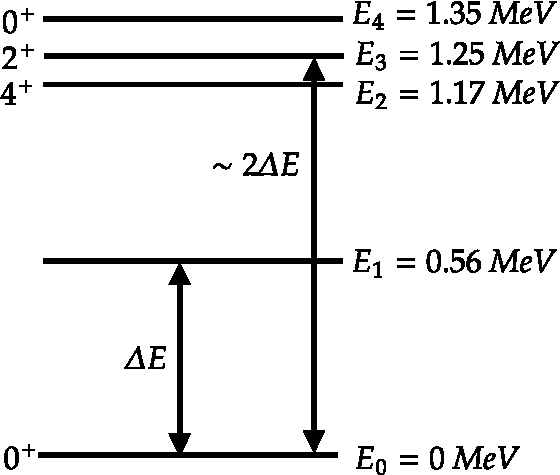
\includegraphics[height=5cm,width=5.5cm]{diagram-20211025-crop}
	\end{figure}
	The spin-parity $j^{p}$ of the level $E_{1}$ is
	{	\exyear{NET/JRF(DEC-2018)}}
	\begin{tasks}(4)
		\task[\textbf{A.}] $1^+$
		\task[\textbf{B.}] $1^-$
		\task[\textbf{C.}] $2^-$
		\task[\textbf{D.}] $2^+$ 
	\end{tasks}
	\item The Bethe-Weizsacker formula for the binding energy (in MeV) of a nucleus of atomic number $Z$ and mass number $A$ is
	$$
	15.8 A-18.3 A^{2 / 3}-0.714 \frac{Z(Z-1)}{A^{1 / 3}}-23.2 \frac{(A-2 Z)^{2}}{A}
	$$
	The ratio $Z / A$ for the most stable isobar of a $A=64$ nucleus, is nearest to
	{	\exyear{NET/JRF(DEC-2019)}}
	\begin{tasks}(4)
		\task[\textbf{A.}] $0.30$
		\task[\textbf{B.}] $0.35$
		\task[\textbf{C.}] $0.45$
		\task[\textbf{D.}] $0.50$
	\end{tasks}
	\item A negative muon, which has a mass nearly 200 times that of an electron, replaces an electron in a $L i$ atom. The lowest ionization energy for the muonic $L i$ atom is approximately
	{	\exyear{NET/JRF(DEC-2019)}}
	\begin{tasks}(2)
		\task[\textbf{A.}] The same as that of $\mathrm{He}$
		\task[\textbf{B.}] The same as that of normal $L i$
		\task[\textbf{C.}]  200 times larger than that of normal $\mathrm{Li}$
		\task[\textbf{D.}]  The same as that of normal $\mathrm{Be}$
	\end{tasks}
	\item The binding energy $B$ of a nucleus is approximated by the formula $B=a_{1} A-a_{2} A^{2 / 3}-a_{3} Z^{2} A^{-1 / 3}-a_{4}(A-2 Z)^{2} A^{-1}$, where $Z$ is the atomic number and $A$ is the mass number of the nucleus. If $\frac{a_{4}}{a_{2}} \simeq 30$. The atomic number $Z$ for naturally stable isobars (constant value of $A$ ) is
	{	\exyear{NET/JRF(JUNE-2020)}}
	\begin{tasks}(4)
		\task[\textbf{A.}]  $\frac{30 A}{60+A^{2 / 3}}$
		\task[\textbf{B.}] $\frac{30 A}{30+A^{2 / 3}}$
		\task[\textbf{C.}]  $\frac{60 A}{120+A^{2 / 3}}$
		\task[\textbf{D.}] $\frac{120 A}{60+A^{2 / 3}}$
	\end{tasks}
	\item The magnetic moments of a proton and a neutron are $2.792 \mu_{N}$ and $-1.913 \mu_{N}$, where $\mu_{N}$ is the nucleon magnetic moment. The values of the magnetic moments of the mirror nuclei ${ }_{9}^{19} F_{10}$ and ${ }_{10}^{19} \mathrm{Ne}_{9}$, respectively, in the Shell model, are closest to
	{	\exyear{NET/JRF(JUNE-2020)}}
	\begin{tasks}(2)
		\task[\textbf{A.}] $23.652 \mu_{N}$ and $-18.873 \mu_{N}$
		\task[\textbf{B.}] $26.283 \mu_{N}$ and $-16.983 \mu_{N}$
		\task[\textbf{C.}] $-2.628 \mu_{N}$ and $1.887 \mu_{N}$
		\task[\textbf{D.}] $2.628 \mu_{N}$ and $-1.887 \mu_{N}$
	\end{tasks}
\end{enumerate}
 \colorlet{ocre1}{ocre!70!}
\colorlet{ocrel}{ocre!30!}
\setlength\arrayrulewidth{1pt}
\begin{table}[H]
	\centering
	\arrayrulecolor{ocre}
	\begin{tabular}{|p{1.5cm}|p{1.5cm}||p{1.5cm}|p{1.5cm}|}
		\hline
		\multicolumn{4}{|c|}{\textbf{Answer key}}\\\hline\hline
		\rowcolor{ocrel}Q.No.&Answer&Q.No.&Answer\\\hline
		1&\textbf{C} &2&\textbf{B}\\\hline 
		3&\textbf{C} &4&\textbf{A} \\\hline
		5&\textbf{C} &6&\textbf{D} \\\hline
		7&\textbf{A}&8&\textbf{C}\\\hline
		9&\textbf{A}&10&\textbf{A}\\\hline
		11&\textbf{B} &12&\textbf{C}\\\hline
		13&\textbf{C}&14&\textbf{A}\\\hline
		15&\textbf{C} &16&\textbf{A} \\\hline
		17&\textbf{A}&18&\textbf{B}\\\hline
		19&\textbf{D}&20&\textbf{C}\\\hline
		21&\textbf{A} &22&\textbf{C}\\\hline
		23&\textbf{D} &&\textbf{} \\\hline
	\end{tabular}
\end{table}
\newpage
\begin{abox}
	Practice Set 2 
\end{abox}
\begin{enumerate}
	\item In the nuclear shell model the spin parity of ${ }_{7}^{15} \mathrm{~N}$ is given by
	{\exyear{GATE 2010}}
	\begin{tasks}(4)
		\task[\textbf{A.}] $\frac{1^{-}}{2}$
		\task[\textbf{B.}] $\frac{1^{+}}{2}$
		\task[\textbf{C.}] $\frac{3^{-}}{2}$
		\task[\textbf{D.}] $\frac{3^{+}}{2}$
	\end{tasks}
	\item The ground state wavefunction of deuteron is in a superposition of $\mathrm{s}$ and $\mathrm{d}$ states. Which of the following is NOT true as a consequence?
	{\exyear{GATE 2010}}
	\begin{tasks}(1)
		\task[\textbf{A.}]  It has a non-zero quadruple moment
		\task[\textbf{B.}] The neutron-proton potential is non-central
		\task[\textbf{C.}]  The orbital wavefunction is not spherically symmetric
		\task[\textbf{D.}]  The Hamiltonian does not conserve the total angular momentum
	\end{tasks}
	\item The first three energy levels of ${ }^{228} T h_{90}$ are shown below\\
	\begin{figure}[H]
		\centering
		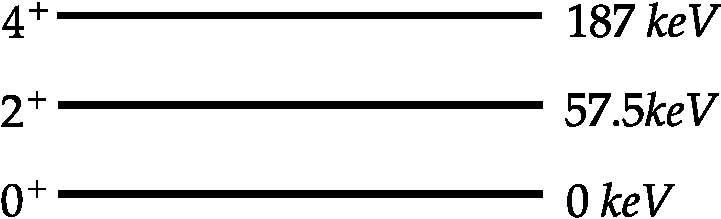
\includegraphics[height=1.5cm,width=6cm]{diagram-20210920-crop}
		\caption{}
		\label{}
	\end{figure}
	The expected spin-parity and energy of the next level are given by
	{\exyear{GATE 2010}}
	\begin{tasks}(4)
		\task[\textbf{A.}] $\left(6^{+} ; 400 \mathrm{keV}\right)$
		\task[\textbf{B.}] $\left(6^{+} ; 300 \mathrm{keV}\right)$
		\task[\textbf{C.}] $\left(2^{+} ; 400 \mathrm{keV}\right)$
		\task[\textbf{D.}] $\left(4^{+} ; 300 \mathrm{keV}\right)$
	\end{tasks}
	\item The semi-empirical mass formula for the binding energy of nucleus contains a surface correction term. This term depends on the mass number $A$ of the nucleus as
	{\exyear{GATE 2011}}
	\begin{tasks}(4)
		\task[\textbf{A.}] $A^{-1 / 3}$
		\task[\textbf{B.}] $A^{1 / 3}$
		\task[\textbf{C.}]  $A^{2 / 3}$
		\task[\textbf{D.}] $A$
	\end{tasks}
	\item According to the single particles nuclear shell model, the spin-parity of the ground state of ${ }_{8}^{17} O$ is
	{\exyear{GATE 2011}}
	\begin{tasks}(4)
		\task[\textbf{A.}] $\frac{1}{2}$
		\task[\textbf{B.}] $\frac{3}{2}$
		\task[\textbf{C.}] $\frac{3^{+}}{2}$
		\task[\textbf{D.}] $\frac{5^{+}}{2}$
	\end{tasks}
	\item In the $\beta$ decay process, the transition $2^{+} \rightarrow 3^{+}$, is
	{\exyear{GATE 2013}}
	\begin{tasks}(1)
		\task[\textbf{A.}] Allowed both by Fermi and Gamow-Teller selection rule
		\task[\textbf{B.}]  Allowed by Fermi and but not by Gamow-Teller selection rule
		\task[\textbf{C.}] Not allowed by Fermi but allowed by Gamow-Teller selection rule
		\task[\textbf{D.}] Not allowed both by Fermi and Gamow-Teller selection rule
	\end{tasks}
	\item Which one of the following is a fermions'?
	{\exyear{GATE 2014}}
	\begin{tasks}(4)
		\task[\textbf{A.}] $\alpha$-particle
		\task[\textbf{B.}] ${ }_{4} B e^{7}$ nucleus
		\task[\textbf{C.}] Hydrogen atom
		\task[\textbf{D.}] Deuteron
	\end{tasks}
	\item The atomic masses of ${ }_{63}^{152} E u,{ }_{62}^{152} \mathrm{Sm},{ }_{1}^{1} H$ and neutron are $151.921749,151.919756$, $1.007825$ and $1.008665$ in atomic mass units (amu), respectively. Using the above information, the $Q$ - value of the reaction ${ }_{63}^{152} E u+n \rightarrow_{62}^{152} S m+p$ is--------------- $\times 10^{-3}$ amu (upto three decimal places)
	{\exyear{GATE 2015}}
	\item In the nuclear shell model, the potential is modeled as $V(r)=\frac{1}{2} m \omega^{2} r^{2}-\lambda \vec{L} \cdot \vec{S}, \lambda>0$. The correct spin-parity and isospin assignments for the ground state of ${ }_{6}^{13} C$ is
	{\exyear{GATE 2015}}
	\begin{tasks}(4)
		\task[\textbf{A.}] $\frac{1^{-}}{2} ; \frac{-1}{2}$
		\task[\textbf{B.}] $\frac{1^{+}}{2} ; \frac{-1}{2}$
		\task[\textbf{C.}] $\frac{3^{+}}{2} ; \frac{1}{2}$
		\task[\textbf{D.}] $\frac{3^{-}}{2} ; \frac{-1}{2}$
	\end{tasks}
	\item According to the nuclear shell model, the respective ground state spin-parity values of ${ }_{8}^{15} O$ and ${ }_{8}^{17} O$ nuclei are
	{\exyear{GATE 2016}}
	\begin{tasks}(4)
		\task[\textbf{A.}] $\frac{1^{+}}{2}, \frac{1^{-}}{2}$
		\task[\textbf{B.}] $\frac{1}{2}^{-}, \frac{5^{+}}{2}$
		\task[\textbf{C.}] $\frac{3^{-}}{2}, \frac{5^{+}}{2}$
		\task[\textbf{D.}] $\frac{3^{-}}{2}, \frac{1^{-}}{2}$
	\end{tasks}
	\item The $\pi^{+}$decays at rest to $\mu^{+}$and $v_{\mu}$. Assuming the neutrino to be massless, the momentum of the neutrino is.................. $\mathrm{MeV} / \mathrm{c}$. (up to two decimal places)\\ $\left(m_{\pi}=139 \mathrm{MeV} / \mathrm{c}^{2}, m_{\mu}=105 \mathrm{MeV} / \mathrm{c}^{2}\right)$
	{\exyear{GATE 2017}}
	\item For nucleus ${ }^{164} \mathrm{Er}$, a $J^{\pi}=2^{+}$state is at $90 \mathrm{keV}$. Assuming ${ }^{164} \mathrm{Er}$ to be a rigid rotor, the energy of its $4^{+}$state is -------------$\mathrm{keV}$ (up to one decimal place)
	{\exyear{GATE 2018}}
\end{enumerate}
 \colorlet{ocre1}{ocre!70!}
\colorlet{ocrel}{ocre!30!}
\setlength\arrayrulewidth{1pt}
\begin{table}[H]
	\centering
	\arrayrulecolor{ocre}
	\begin{tabular}{|p{1.5cm}|p{1.5cm}||p{1.5cm}|p{1.5cm}|}
		\hline
		\multicolumn{4}{|c|}{\textbf{Answer key}}\\\hline\hline
		\rowcolor{ocrel}Q.No.&Answer&Q.No.&Answer\\\hline
		1&\textbf{B} &2&\textbf{D}\\\hline 
		3&\textbf{A} &4&\textbf{C} \\\hline
		5&\textbf{D} &6&\textbf{C} \\\hline
		7&\textbf{B}&8&\textbf{2.833}\\\hline
		9&\textbf{A}&10&\textbf{B}\\\hline
		11&\textbf{29.84} &12&\textbf{300}\\\hline
	\end{tabular}
\end{table}
\newpage
\begin{abox}
	Practice Set 3 
\end{abox}
\begin{enumerate}
	\item Two spherical nuclei have mass numbers 216 and 64 with their radii $R_{1}$ and $R_{2}$, respectively. The ratio $\frac{R_{1}}{R_{2}}$ is
	{	\exyear{IIT JAM 2009}}
	\begin{tasks}(4)
		\task[\textbf{A.}]1
		\task[\textbf{B.}]1.5
		\task[\textbf{C.}]2
		\task[\textbf{D.}]2.5
	\end{tasks}
	\item The variation of binding energy per nucleon with respect to the mass number of nuclei is shown in the figure.
	Consider the following reactions:
	(i) ${ }_{92}^{238} U \rightarrow_{82}^{206} P b+10 P+22 n$
	(ii) ${ }_{92}^{238} \mathrm{U} \rightarrow{ }_{82}^{206} \mathrm{~Pb}+8{ }_{2}^{4} \mathrm{He}+6 e^{-}$
	Which one of the following statements is true for the given decay modes of ${ }_{92}^{238} U$ ?
	{\exyear{IIT JAM 2015}}
	\begin{figure}[H]
		\centering
		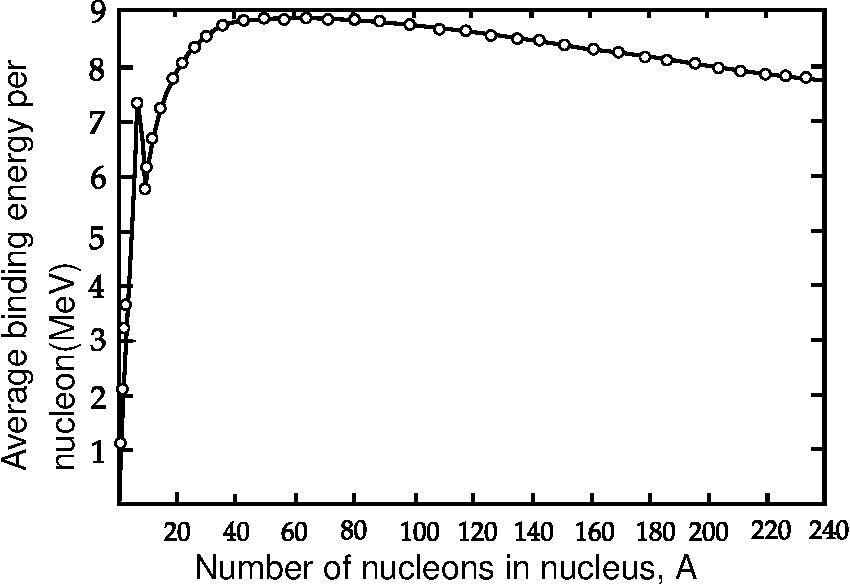
\includegraphics[height=5cm,width=8cm]{diagram-20211122(45)-crop}
	\end{figure}
	\begin{tasks}(2)
		\task[\textbf{A.}]Both (i) and (ii) are allowed
		\task[\textbf{B.}]Both (i) and (ii) are forbidden
		\task[\textbf{C.}](i) is forbidden and (ii) is allowed
		\task[\textbf{D.}](i) is allowed and (ii) is forbidden
	\end{tasks}
	\item For an atomic nucleus with atomic number $Z$ and mass number $A$, which of the following is (are) correct?
	{	\exyear{IIT JAM 2017}}
	\begin{tasks}(1)
		\task[\textbf{A.}](a) Nuclear matter and nuclear charge are distributed identically in the nuclear volume
		\task[\textbf{B.}]Nuclei with $Z>83$ and $A>209$ emit $\alpha$ - radiation
		\task[\textbf{C.}] The surface contribution to the binding energy is proportional to $A^{2 / 3}$
		\task[\textbf{D.}]$\beta$ - decay occurs when the proton to neutron ratio is large, but not when it is small
	\end{tasks}
	\item The relation between the nuclear radius $(R)$ and the mass number $(A)$, given by $R=1.2 A^{1 / 3} \mathrm{fm}$, implies that
	{	\exyear{IIT JAM 2019}}
	\begin{tasks}(1)
		\task[\textbf{A.}]The central density of nuclei is independent of $A$
		\task[\textbf{B.}]The volume energy per nucleon is a constant
		\task[\textbf{C.}]The attractive part of the nuclear force has a long range
		\task[\textbf{D.}]The nuclear force is charge dependent
	\end{tasks}
	\item A duetron strikes ${ }_{8} \mathrm{O}^{16}$ nucleus with subsequent emission of alpha particle. Identify the nucleus so produced
	\begin{tasks}(2)
		\task[\textbf{A.}] ${ }_{3} \mathrm{Li}^{7}$
		\task[\textbf{B.}]  ${ }_{5} \mathrm{~B}^{10}$
		\task[\textbf{C.}]${ }_{7} \mathrm{~N}^{13}$
		\task[\textbf{D.}]${ }_{7} \mathrm{~N}^{14}$
	\end{tasks}
	\item For a nuclear fusion process, suitable nuclei are
	\begin{tasks}(2)
		\task[\textbf{A.}]any Nuclei 
		\task[\textbf{B.}] heavy Nuclei
		\task[\textbf{C.}]light Nuclei
		\task[\textbf{D.}]nuclei lying in the middle of periodic table
	\end{tasks}
	\item A nuclear reaction is given by $\mathrm{Z}^{\mathrm{X}}{\mathrm{A}} \rightarrow \mathrm{Z}_{+1} \mathrm{Y}^{\mathrm{A}}+{ }_{-1} \mathrm{e}^{0}+\bar{v}$, represents
	\begin{tasks}(2)
		\task[\textbf{A.}] fission
		\task[\textbf{B.}] $\beta$-decay
		\task[\textbf{C.}]$\sigma$-decay
		\task[\textbf{D.}]fusion
	\end{tasks}
	\item A nucleus ${ }_{n}^{m} X$ emits one $\alpha$-particle and two $\beta$-particles. The resulting nucleus is
	\begin{tasks}(1)
		\task[\textbf{A.}] $\underset{\mathrm{n}-4}{\mathrm{~m}-6} \mathrm{Z}$
		\task[\textbf{B.}] $\underset{\mathrm{n}}{\mathrm{m}-6} \mathrm{Z}$
		\task[\textbf{C.}]${ }_{\mathrm{n}}^{\mathrm{m}-4} \mathrm{X}$
		\task[\textbf{D.}]${ }_{\mathrm{n}-2}^{\mathrm{m}-4} \mathrm{Y}$
	\end{tasks}
	\item The mass of a ${ }_{3}^{7} L i$ nucleus is $0.042 \mathrm{u}$ less than the sum of the masses of all its nucleons. The binding energy per nucleon of ${ }_{3}^{7} L i$ nucleus is nearly
	\begin{tasks}(2)
		\task[\textbf{A.}]$46 \mathrm{MeV}$
		\task[\textbf{B.}] $5.6 \mathrm{MeV}$
		\task[\textbf{C.}]$3.9 \mathrm{MeV}$
		\task[\textbf{D.}]$23 \mathrm{MeV}$ 
	\end{tasks}		
	\item A nucleus disintegrated into two nuclear parts which have their velocities in the ratio of $2: 1$. The ratio of their nuclear sizes will be
	\begin{tasks}(2)
		\task[\textbf{A.}]  $3^{1 / 2}: 1$
		\task[\textbf{B.}]  $1: 2^{1 / 3}$
		\task[\textbf{C.}]$2^{1 / 3}: 1$
		\task[\textbf{D.}]$1: 3^{1 / 2}$
	\end{tasks}	
\end{enumerate}